\documentclass[mstat,12pt]{unswthesis}





%%%%%%%%%%%%%%%%%%%%%%%%%%%%%%%%%%%%%%%%%%%%%%%%%%%%%%%%%%%%%%%%%%
% 
% OK...Now we get to some actual input.  The first part sets up
% the title etc that will appear on the front page
%
%%%%%%%%%%%%%%%%%%%%%%%%%%%%%%%%%%%%%%%%%%%%%%%%%%%%%%%%%%%%%%%%%

\title{Capstone Project by Team Group K\\[0.5cm]Forecasting Energy
Demand in New South Wales: An Analysis of Temperature, Regional
Reference Price, Holidays, and Time Series Data, with an Examination of
Demand in Relation to Population Growth}

\authornameonly{Abdelrhman Dameen (z5427841), Md Nezam Uddin
(z5339862), Pam Moodley (z5366156), Van Hai Ho (z3071030) }

\author{\Authornameonly}

\copyrightfalse
\figurespagefalse
\tablespagefalse

%%%%%%%%%%%%%%%%%%%%%%%%%%%%%%%%%%%%%%%%%%%%%%%%%%%%%%%%%%%%%%%%%
%
%  And now the document begins
%  The \beforepreface and \afterpreface commands puts the
%  contents page etc in
%
%%%%%%%%%%%%%%%%%%%%%%%%%%%%%%%%%%%%%%%%%%%%%%%%%%%%%%%%%%%%%%%%%%


%%%%%%%%%%%%%%%%%%%%%%%%%%%%%%%%%%%%%%%%%%%%%%%%%%%%%%%%%%%%%%%%%%%%%%%
%
%  A small sample UNSW Coursework Masters thesis file.
%  Any questions to Ian Doust i.doust@unsw.edu.au and/or Gery Geenens ggeenens@unsw.edu.au
%
%%%%%%%%%%%%%%%%%%%%%%%%%%%%%%%%%%%%%%%%%%%%%%%%%%%%%%%%%%%%%%%%%%%%%%%
%
%  The first part pulls in a UNSW Thesis class file.  This one is
%  slightly nonstandard and has been set up to do a couple of
%  things automatically
%
 
%%%%%%%%%%%%%%%%%
%% Precisely one of the next four lines should be uncommented.
%% Choose the one which matches your degree, uncomment it, and comment out the other two!
%\documentclass[mfin,12pt]{unswthesis}    %%  For Master of Financial Mathematics 
%\documentclass[mmath,12pt]{unswthesis}   %%  For Master of Mathematics
%\documentclass[mstat,12pt]{unswthesis}  %%  For Master of Statistics
%%%%%%%%%%%%%%%%%



\linespread{1}
\usepackage{amsfonts}
\usepackage{amssymb}
\usepackage{amsthm}
\usepackage{latexsym,amsmath}
\usepackage{graphicx}
\usepackage{afterpage}
\usepackage[colorlinks]{hyperref}
 \hypersetup{
     colorlinks=true,
     linkcolor=blue,
     filecolor=blue,
     citecolor= black,      
     urlcolor=cyan,
     }
\usepackage{textcomp}
\usepackage{longtable}
\usepackage{booktabs}
\usepackage{float}

%%%%%%%%%%%%%%%%%%%%%%%%%%%%%%%%%%%%%%%%%%%%%%%%%%%%%%%%%%%%%%%%%
%
%  The following are some simple LaTeX macros to give some
%  commonly used letters in funny fonts. You may need more or less of
%  these
%
\newcommand{\R}{\mathbb{R}}
\newcommand{\Q}{\mathbb{Q}}
\newcommand{\C}{\mathbb{C}}
\newcommand{\N}{\mathbb{N}}
\newcommand{\F}{\mathbb{F}}
\newcommand{\PP}{\mathbb{P}}
\newcommand{\T}{\mathbb{T}}
\newcommand{\Z}{\mathbb{Z}}
\newcommand{\B}{\mathfrak{B}}
\newcommand{\BB}{\mathcal{B}}
\newcommand{\M}{\mathfrak{M}}
\newcommand{\X}{\mathfrak{X}}
\newcommand{\Y}{\mathfrak{Y}}
\newcommand{\CC}{\mathcal{C}}
\newcommand{\E}{\mathbb{E}}
\newcommand{\cP}{\mathcal{P}}
\newcommand{\cS}{\mathcal{S}}
\newcommand{\A}{\mathcal{A}}
\newcommand{\ZZ}{\mathcal{Z}}
%%%%%%%%%%%%%%%%%%%%%%%%%%%%%%%%%%%%%%%%%%%%%%%%%%%%%%%%%%%%%%%%%%%%%
%
% The following are much more esoteric commands that I have left in
% so that this file still processes. Use or delete as you see fit
%
\newcommand{\bv}[1]{\mbox{BV($#1$)}}
\newcommand{\comb}[2]{\left(\!\!\!\begin{array}{c}#1\\#2\end{array}\!\!\!\right)
}
\newcommand{\Lat}{{\rm Lat}}
\newcommand{\var}{\mathop{\rm var}}
\newcommand{\Pt}{{\mathcal P}}
\def\tr(#1){{\rm trace}(#1)}
\def\Exp(#1){{\mathbb E}(#1)}
\def\Exps(#1){{\mathbb E}\sparen(#1)}
\newcommand{\floor}[1]{\left\lfloor #1 \right\rfloor}
\newcommand{\ceil}[1]{\left\lceil #1 \right\rceil}
\newcommand{\hatt}[1]{\widehat #1}
\newcommand{\modeq}[3]{#1 \equiv #2 \,(\text{mod}\, #3)}
\newcommand{\rmod}{\,\mathrm{mod}\,}
\newcommand{\p}{\hphantom{+}}
\newcommand{\vect}[1]{\mbox{\boldmath $ #1 $}}
\newcommand{\reff}[2]{\ref{#1}.\ref{#2}}
\newcommand{\psum}[2]{\sum_{#1}^{#2}\!\!\!'\,\,}
\newcommand{\bin}[2]{\left( \begin{array}{@{}c@{}}
				#1 \\ #2
			\end{array}\right)	}
%
%  Macros - some of these are in plain TeX (gasp!)
%
\newcommand{\be}{($\beta$)}
\newcommand{\eqp}{\mathrel{{=}_p}}
\newcommand{\ltp}{\mathrel{{\prec}_p}}
\newcommand{\lep}{\mathrel{{\preceq}_p}}
\def\brack#1{\left \{ #1 \right \}}
\def\bul{$\bullet$\ }
\def\cl{{\rm cl}}
\let\del=\partial
\def\enditem{\par\smallskip\noindent}
\def\implies{\Rightarrow}
\def\inpr#1,#2{\t \hbox{\langle #1 , #2 \rangle} \t}
\def\ip<#1,#2>{\langle #1,#2 \rangle}
\def\lp{\ell^p}
\def\maxb#1{\max \brack{#1}}
\def\minb#1{\min \brack{#1}}
\def\mod#1{\left \vert #1 \right \vert}
\def\norm#1{\left \Vert #1 \right \Vert}
\def\paren(#1){\left( #1 \right)}
\def\qed{\hfill \hbox{$\Box$} \smallskip}
\def\sbrack#1{\Bigl \{ #1 \Bigr \} }
\def\ssbrack#1{ \{ #1 \} }
\def\smod#1{\Bigl \vert #1 \Bigr \vert}
\def\smmod#1{\bigl \vert #1 \bigr \vert}
\def\ssmod#1{\vert #1 \vert}
\def\sspmod#1{\vert\, #1 \, \vert}
\def\snorm#1{\Bigl \Vert #1 \Bigr \Vert}
\def\ssnorm#1{\Vert #1 \Vert}
\def\sparen(#1){\Bigl ( #1 \Bigr )}

\newcommand\blankpage{%
    \null
    \thispagestyle{empty}%
    \addtocounter{page}{-1}%
    \newpage}

%%%%%%%%%%%%%%%%%%%%%%%%%%%%%%%
%
% These environments allow you to get nice numbered headings
%  for your Theorems, Definitions etc.  
%
%  Environments
%
%%%%%%%%%%%%%%%%%%%%%%%%%%%%%%%

\newtheorem{theorem}{Theorem}[section]
\newtheorem{lemma}[theorem]{Lemma}
\newtheorem{proposition}[theorem]{Proposition}
\newtheorem{corollary}[theorem]{Corollary}
\newtheorem{conjecture}[theorem]{Conjecture}
\newtheorem{definition}[theorem]{Definition}
\newtheorem{example}[theorem]{Example}
\newtheorem{remark}[theorem]{Remark}
\newtheorem{question}[theorem]{Question}
\newtheorem{notation}[theorem]{Notation}
\numberwithin{equation}{section}

%%%%%%%%%%%%%%%%%%%%%%%%%%%%%%%%%%%%%%%%%%%%%%%%%%%%%%%%%%%%%%%%%%
%
%  If you've got some funny special words that LaTeX might not
% hyphenate properly, you can give it a helping hand:
%

\hyphenation{Mar-cin-kie-wicz Rade-macher}


\newlength{\cslhangindent}
\setlength{\cslhangindent}{1.5em}
\newlength{\csllabelwidth}
\setlength{\csllabelwidth}{3em}
\newenvironment{CSLReferences}[2] % #1 hanging-ident, #2 entry spacing
 {% don't indent paragraphs
  \setlength{\parindent}{0pt}
  % turn on hanging indent if param 1 is 1
  \ifodd #1 \everypar{\setlength{\hangindent}{\cslhangindent}}\ignorespaces\fi
  % set entry spacing
  \ifnum #2 > 0
  \setlength{\parskip}{#2\baselineskip}
  \fi
 }%
 {}
\usepackage{calc} % for \widthof, \maxof
\newcommand{\CSLBlock}[1]{#1\hfill\break}
\newcommand{\CSLLeftMargin}[1]{\parbox[t]{\maxof{\widthof{#1}}{\csllabelwidth}}{#1}}
\newcommand{\CSLRightInline}[1]{\parbox[t]{\linewidth}{#1}}
\newcommand{\CSLIndent}[1]{\hspace{\cslhangindent}#1}

\bibliographystyle{elsarticle-num}




\begin{document}

\beforepreface

%\afterpage{\blankpage}

% plagiarism

\prefacesection{Plagiarism statement}

\vskip 2pc \noindent I declare that this thesis is my
own work, except where acknowledged, and has not been submitted for
academic credit elsewhere. 

\vskip 2pc  \noindent I acknowledge that the assessor of this
thesis may, for the purpose of assessing it:
\begin{itemize}
\item Reproduce it and provide a copy to another member of the University; and/or,
\item Communicate a copy of it to a plagiarism checking service (which may then retain a copy of it on its database for the purpose of future plagiarism checking).
\end{itemize}

\vskip 2pc \noindent I certify that I have read and understood the University Rules in
respect of Student Academic Misconduct, and am aware of any potential plagiarism penalties which may 
apply.\vspace{24pt}

\vskip 2pc \noindent By signing 
this declaration I am
agreeing to the statements and conditions above.
\vskip 2pc \noindent
Signed: \rule{7cm}{0.25pt} \hfill Date: \rule{4cm}{0.25pt} \\[1cm]
Signed: \rule{7cm}{0.25pt} \hfill Date: \rule{4cm}{0.25pt} \\[1cm]
Signed: \rule{7cm}{0.25pt} \hfill Date: \rule{4cm}{0.25pt} \\[1cm]
Signed: \rule{7cm}{0.25pt} \hfill Date: \rule{4cm}{0.25pt} \\[1cm]
\vskip 1pc

%\afterpage{\blankpage}

% Acknowledgements are optional


\prefacesection{Acknowledgements}

{\bigskip}We would like to express our sincere gratitude to several
individuals and organizations for supporting us throughout this project.
First, we wish to express our sincere gratitude to our supervisors,
Sarat Moka, Wei Tian, and Armin Chitizadeh for their enthusiasm,
patience, insightful comments, helpful information, practical advice and
unceasing ideas that have helped us tremendously at all times in our
research and writing of this report. Their immense knowledge, profound
experience and professional expertise in analysis Quality Control has
enabled us to complete this research successfully. Without their support
and guidance, this project would not have been possible. We could not
have imagined having better supervisors in our study.\\[1cm] We are also
grateful to the following Group K team members: Abdelrhman Dameen, Md
Nezam Uddin, Pam Moodley, and Van Hai Ho for their consistent support
and assistance.\\[1cm] Finally, last but by no means least; also to
everyone in Endgame Economics for providing the dataset and for the
great insights, time, and effort especially Oliver Nunn and Dr.~Jack
Simpson.\\[1cm] Thanks for all your encouragement!\\[1cm] 

{\bigskip\bigskip\bigskip\noindent} 07 October, 2023.

%\afterpage{\blankpage}

% Abstract

\prefacesection{Abstract}

{\bigskip}This research report investigates the factors influencing
energy demand in New South Wales, with an emphasis on variables such as
temperature, price, holidays, and time-series data. The study also
examines the relationship between energy demand and population
growth.\\[1cm] Energy demand forecasting is essential for maintaining a
sustainable energy infrastructure and for policy planning. With the
challenges posed by climate change and urbanization, precise forecasting
models are increasingly crucial for efficient energy resource
management.\\[1cm] Despite various models exploring energy demand, few
studies comprehensively analyze how specific factors such as regional
reference prices and holidays impact demand, and even fewer examine
these in relation to population growth in New South Wales. How do
temperature, prices, holidays, and population growth impact energy
demand in New South Wales? Can machine learning models effectively
forecast energy demand?\\[1cm] A variety of machine learning algorithms
were employed, including Linear Regression, Multi-Layer Perceptron,
Random Forest, Facebook Prophet, and XGBoost. These models were assessed
using metrics such as MAPE, MAE, and RMSE. Machine learning models,
particularly XGBoost, can offer nuanced and effective forecasts of
energy demand. Time-series data, regional reference prices, holidays,
and population trends are significant variables influencing energy
demand. Among the models used, XGBoost showed the best performance with
a 7\% MAPE score.\\[1cm] Factors such as temperature, price of energy,
and holidays are significant predictors. This research enhances our
understanding of the multifaceted factors affecting energy demand in New
South Wales. It demonstrates that machine learning algorithms,
especially ensemble models such as XGBoost, can be powerful tools in
energy demand forecasting. By acknowledging the importance of regional
factors such as population growth and holidays, this study contributes
to more accurate and region-specific energy demand models.\\[1cm] 

%\afterpage{\blankpage}


\afterpreface





%%%%%%%%%%%%%%%%%%%%%%%%%%%%%%%%%%%%%%%%%%%%%%%%%%%%%%%%%%%%%%%%%%
%
% Now we can start on the first chapter
% Within chapters we have sections, subsections and so forth
%
%%%%%%%%%%%%%%%%%%%%%%%%%%%%%%%%%%%%%%%%%%%%%%%%%%%%%%%%%%%%%%%%%%



%%%%%%%%%%%%%%%%%%%%%%%%%%%%%%%%%%%%%

%\afterpage{\blankpage}


\hypertarget{s-introduction}{%
\chapter{Introduction}\label{s-introduction}}

The volatility of energy supply and demand poses a challenge for
suppliers to enter and remain profitable in the market. Accurately
predicting and efficiently supplying energy to the grid is critical for
profitability. A key determinant of energy demand is weather; heating is
necessary when temperatures drop, and air conditioning becomes essential
as temperatures rise. Therefore, this analysis aims to examine the
influence of weather on energy demand, considering the significant
effects of global warming and erratic weather patterns.

However, other variables also come into play. As the International
Atomic Energy Agency suggests, ``The analysis should be conducted with
relevant and consistent macroeconomic and microeconomic data, so that
electricity demand projections can be more reliable and consistent with
demographic, economic and industrial development projections'' (IEA
(2016)). This sentiment is further echoed by Emami Javanmard and Ghaderi
who state, ``The increase in population and economic growth of countries
has led to a rise in energy consumption, which has created several
challenges and problems for governments and nations'' (Emami Javanmard
and Ghaderi (2023)).

Considering these challenges, the project will explore daily and
seasonal variations, as well as the impact of holidays on energy demand.
By incorporating these factors, we intend to highlight the benefits of
using machine learning models for more efficient demand prediction, a
point also emphasized by a report stating, ``The demand for energy
continues to grow as the world's population increases. And to ensure we
meet these demands, utility and energy companies need reliable energy
demand forecasting'' (U.S Energy Information Administration (2020)).

Specifically, we will uncover hidden temporal trends in demand,
including daily and seasonal fluctuations, through the identification of
energy consumption patterns. ``According to the Global Energy
Statistical website, energy consumption worldwide has increased by
approximately 70\% from 1990 to 2020'' (Perle (2023)). We will try to
understand how variables such as temperature impact energy demand.
Furthermore, we will analyze the effect of holidays and special events
on demand, aiding better planning efforts.

In New South Wales, the government anticipates exponential population
growth, but this prediction may not sufficiently account for the
intertwined relationship between energy resources and population
capacity.

As populations grow, the demand for energy escalates, putting strain on
existing resources. This can make energy sources scarcer and more
difficult to extract, exemplified by the need to mine deeper for coal or
explore complex environments for oil. The scarcity leads to declining
marginal returns in energy extraction, pushing the quest for new energy
sources. These new sources, in turn, can expand the Earth's carrying
capacity, enabling further population growth.

Therefore, the correlation between energy availability and population
size could imply that if energy resources are nearing their peak
production rates, New South Wales might also be approaching its maximum
sustainable population. Hence, planning for the future should factor in
these variables to create more accurate and sustainable growth
forecasts. ``In economies experiencing rapid residential electricity
consumption and burgeoning energy-intensive activities, there is a
notable link between economic growth and electricity use. Specifically,
in less developed non-OECD countries, per capita electricity growth more
than doubled from 2000 to 2017. This is in stark contrast to the nearly
flat trend observed in more developed OECD countries'' (Wolde-Rufael
(2006)).

We hypothesize that growing population correlates with increasing energy
demand. To confirm or refute this, we will perform an analysis that may
also reveal other influential factors. Consequent to our analysis,
policy recommendations will be provided to aid in energy policy
formulation, including diversification of energy sources to meet demand.
We aim to develop a machine learning model capable of predicting future
energy demand with high accuracy, incorporating all the identified
variables.

Electricity demand forecasting is an indispensable tool for managing the
power grid and ensuring a reliable supply. It is a complex task,
influenced by a multitude of factors. While traditional forecasting
methods have their merits, there is growing interest in employing
machine learning algorithms such as Linear Regression, Random Forest,
and XG Boost for more accurate predictions.

For model performance evaluation, metrics such as Root Mean Square Error
(RMSE), Mean Absolute Error (MAE), and Mean Absolute Percentage Error
(MAPE) will be used, given the time-dependent nature of the data. These
metrics will serve as complementary tools for a comprehensive evaluation
of our forecasting models.

Two common approaches to forecasting energy demand are top-down and
bottom-up. The top-down approach focuses on macro factors such as the
economy, population growth, and weather, while the bottom-up approach
examines energy consumption at the individual or company level. Both
methods contribute to understanding future energy needs.

The subsequent sections of this report are organized as follows: Chapter
\ref{s-literature-review} presents a literature review, establishing the
relevance and importance of our study for policymakers in New South
Wales and the energy sector. Chapter \ref{s-material-methods} elaborates
on the methods, machine learning algorithms, and evaluation benchmarks.
Chapter \ref{s-data-analysis} delves into the data, exploring
descriptive statistics and outlier analysis, prepares the data for the
main model and explores various visual plots, examines the relationship
between total demand and the estimated population of New South Wales.
Chapter \ref{s-analysis-results} analyzes and compares the results to
other metrics, while Chapter \ref{s-discussion} discusses these results.
Finally, Chapter \ref{s-conclusion} concludes the report, offering
recommendations and addressing further issues.

\hypertarget{s-literature-review}{%
\chapter{Literature Review}\label{s-literature-review}}

When looking at the previous studies, papers and approaches for
electricity demand forecast we discovered the use of different methods
manual and automated, techniques in a way of forecasting energy demand,
some of them addressed more ML methods. Other studies examined the broad
applications of ML in energy system. Our unique focus on Demand in NSW
electrical demand prediction offers deeper understanding, to the point
of challenging conventional wisdom about things such as the connection
between pricing and temperature and the relationship between population
increase and forecast issues. It is important to note, however, that we
discuss deeper ways in which grid search is used to find the optimal
model, in addition to pure applications of some benchmark measures to
analyse the performance of our primary model.

In his paper (Graham Zabel (2009)), Graham Zabel examines the
sum-of-energies concept in relation to population expansion,
highlighting its broad-reaching ramifications. Zabel acknowledges a
number of aspects, including population control and natural
catastrophes, but contends that energy resources have an indirect
influence on these concerns. Instead of going into depth on particular
energy sources such as nuclear or hydroelectricity, the study primarily
focuses on the significance of fossil fuels in influencing world
population trends. According to Zabel, determining Earth's carrying
capacity requires a knowledge of the interactions between energy
resources and population development.

The 2023 paper by Pelka (Pawel Pelka (2023)), titled ``Analysis and
Forecasting of Monthly Electricity Demand Time Series Using
Pattern-Based Statistical Methods,'' focuses on the vital duty of
precisely predicting monthly electricity load (MEL). Given that energy
must be produced in real-time, the article, which was published in
Energies, emphasises the significance of exact projections for
sustaining affordable and dependable power systems. Pelka investigates a
range of forecasting models, including traditional techniques, neural
networks, and deep learning. In order to make complicated interactions
between variables easier to understand, the study introduces the use of
pattern representation in statistical approaches. Additionally, it
emphasises how crucial it is to comprehend stationary time series in
order to make precise predictions. The paper analyses data from Poland
and 35 European nations to highlight the difficulties in MEL time series
data, including non-linear trends and seasonal changes.

Writing for the U.S. Energy Information Administration Ari Kahan (IEA
(2016)) states the world's power consumption is growing faster than its
population. The emerging, non-OECD nations where the per capita power
usage more than quadrupled between 2000 and 2017 are where this trend is
most pronounced. In contrast, the use of energy has mostly followed a
flat trend in industrialised OECD nations. Improvements in lighting
technology and other efficiency measures have helped to somewhat offset
this increase in usage. Kahan points out that in less developed
countries, using more electricity per person is directly tied to
economic growth. However, this isn't necessarily true for big,
industrialized nations. Using the United States as an example, where per
capita energy usage differs significantly from state to state, he also
notices notable within-country variations.

In their recent paper from 2023 titled ``Energy demand forecasting in
seven sectors by an optimization model based on machine learning
algorithms,'' Majid Emami Javanmard and S.F. Ghaderi (Majid Emami
Javanmard, S.F. Ghaderi (2023)) explored long-term forecasting energy
demand in Iran up to 2040. They employed a range of machine learning
algorithms, including ANN, AR, ARIMA, SARIMA, SARIMAX, and LSTM, and
integrated them with mathematical programming. In especially for Iran,
the study emphasises the urgent problem of rising energy demand as
people and economies expand. To improve their integrated model, the
authors carefully assess the forecast accuracy of each algorithm in each
industry. By providing a multi-algorithmic approach that takes into
consideration the intricacies and variances of many sectors, this study
adds to the body of literature already in existence. Additionally, they
assess the performance of their integrated model using five criteria for
prediction accuracy, demonstrating that their approach yields
predictions that are more accurate than those produced by independent
machine learning methods.

Shereen Elsayed, Daniela Thyssens, Ahmed Rashed, Hadi Samer Jomaa, and
Lars Schmidt-Thieme (Elsayed, S, Thyssens, D, Rashed, A, Jomaa, HS \&
Schmidt-Thieme, L (2021)) demonstrate in their recent 2021 paper titled
``Do We Really Need Deep Learning Models for Time Series Forecasting?''
that XGBoost outperforms deep learning models for time series
forecasting. They also prove that time series forecasting has a long
history of simple models, such as exponential smoothing and linear
models, outperforming more complicated ones. The paper presents several
assertive statements that bear resemblance to assertions in the realm of
scientific discourse, rather than embodying a strictly objective pursuit
of knowledge.

\begin{enumerate}
\def\labelenumi{\arabic{enumi}.}
\item
  The paper claims that GBRT predictions outperform ``state-of-the-art''
  neural forecasting methods, most of which are five years old, casting
  doubt on the seriousness of all their experiments. In the authors'
  words: ``Stronger transformer-based models, such as the temporal
  fusion transformer, rightfully surpass the boosted regression tree.''
\item
  It is suspiciously convenient that all nine benchmark datasets
  considered in the experiments are high-frequency.
\end{enumerate}

Recently the government of NSW introduced a energy efficient program it
started in 2009 and will run until 2050. (Minister for Planning and
Public Spaces (2023)) These incentives give businesses and residents who
own a home as well as companies financial incentives to upgrade their
appliances and power outlets to a more energy-efficient one.\\
The state construction codes have also been changed to ensure that all
newly constructed homes have better and more effective energy ratings,
which will lower the need for electricity even if the population is
continuously growing.

Our analysis aims to establish a generalized model for forecasting
energy demands in NSW, which has both long-term and short-term
forecasting implications. and it uses a grid\_search model to look for
the best model and It employs multi-objective models that consider
various machine learning algorithms to improve forecasting accuracy. It
aims to provide energy suppliers and policymakers with valuable insights
for better demand management, thus ensuring a stable and reliable energy
supply for the NSW population.

\hypertarget{s-material-methods}{%
\chapter{Material and Methods}\label{s-material-methods}}

\hypertarget{software}{%
\section{Software}\label{software}}

Python, R/RSudio, and Jupyter Notebook software are used to Analyse the
data. Libraries and packages such as pandas, matplotlib, seaborn for
Python and ggplot2, dplyr, caret for R are required in this analysis.
RMarkdown, knitr are also utilized for putting the analysis together.

Scikit-learn is a machine learning library in Python, widely used in
this analysis. The algorithms we used for forecasting such as Linear
Regression, Multi-Layer Perceptron, Random Forest and XGBoost are all
available in scikit-learn library.

For project management, cloud storage, version control and code
collaboration GitHub gave us pro level access as a student.

\hypertarget{description-of-the-data}{%
\section{Description of the Data}\label{description-of-the-data}}

We will use the provided data sets as our core data for our analysis,
including:

\begin{itemize}
\item
  \emph{totaldemand\_nsw.csv}: Total Demand data.
\item
  \emph{temperature\_nsw.csv}: Temperature data.
\end{itemize}

The data will need further analysis and cleaning, including the removal
of invalid and outlier data before being utilised to generate the demand
forecast.

\hypertarget{total-demand-data}{%
\subsection{Total Demand data}\label{total-demand-data}}

The Total Demand data provided in file \emph{totaldemand\_nsw.csv}
contains energy demand in 5-minute intervals from January 1, 2010, to
August 1, 2022, for New South Wales. The data is in a comma-delimited
file format, with columns labeled Datetime, RegionId, and TotalDemand.
The RegionId consists only of NSW1, which indicated there would not be a
need to filter the data.

\hypertarget{temperature-data}{%
\subsection{Temperature data}\label{temperature-data}}

The temperature data provided in file \emph{temperature\_nsw.csv} is in
30-minute intervals from January 1, 2010, to August 1, 2022, for New
South Wales. The data is provided in a comma-delimited file format, with
headings DateTime, Location, and Temperature (in Celsius). The source of
the temperature data is the Bankstown weather location which is in New
South Wales.

\hypertarget{nsw-public-holidays}{%
\subsection{NSW Public Holidays}\label{nsw-public-holidays}}

We seek to ascertain whether public holidays would impact the energy
demand and what is the pattern and relationship with energy demand. New
Sout Wales public holiday data is publicly available from NSW Government
Industrial Relations website.

The data source was manually captured from the different sources, and
therefore were in different formats. One file was created for each year
to ensure it was simpler to track which years were needed to be found
and captured.

\hypertarget{aggregated-price-and-demand-data}{%
\subsection{Aggregated Price and Demand
Data}\label{aggregated-price-and-demand-data}}

The Energy price is another factor affecting the energy demand. We use
the aggregated price and demand data publicly available at Australian
Energy Market Operator (AEMO) website (Australian Energy Market Operator
({[}no date{]})).

Aggregated Price and Demand data is available per month from the year
1998 to the current month. For the purpose of this project, we
downloaded data for the year 2010 to 2022. This accounted to 156 data
files being downloaded to integrate with the total demand and
temperature data sets. These data files are merged into a single file in
the same format with the following headers:

\begin{itemize}
\tightlist
\item
  REGION: NSW Region.
\item
  SETTLEMENTDATE: Settlement date and time for every 5 minutes.
\item
  TOTALDEMAND: Total demand at the settlement date and time.
\item
  RRP: Retail Price.
\item
  PERIODTYPE: Period Type.
\end{itemize}

From this data set, only the settlement date and RRP was utilised.

\hypertarget{population-data}{%
\subsection{Population Data}\label{population-data}}

We hypothesised as population grows, the demand for energy increases.
Analysis was done to understand if our hyphothesis is true; or false,
and what other factors might influence the energy demand. Population
data that we use is publicly available at Australian Bureau of
Statistics (Australian Bureau of Statistics ({[}no date{]})). This data
is used in our analysis and is available in our repository:
\url{https://github.com/van-hai-ho/ZZSC9020_Project_Group_K/blob/main/data/NSW\%20estimated\%20population.xlsx}.

\hypertarget{data-set-format}{%
\subsection{Data set format}\label{data-set-format}}

All the data sets, i.e.~Temperature, Energy Demand, Energy Price,
Holidays, and Population is integrated before continuing. When merging
these data sets, there is a mismatch in frequency since the demand is in
5-minute intervals and the temperature data is in 30-minute intervals.
There are approximately 1.3 million rows of demand data and 247,646 rows
of temperature data. When merging the temperature and demand data, the
demand data is grouped into 30 minute intervals and the mean is
calculated and utilised when merged with the temperature data.

Since this project aims to address questions regarding future energy
demand, historical data will be utilized, and the initial data sets
provided are an excellent starting point. Additional data will be
sourced to enhance these data sets.

As we hypothesised that the energy demand would increase when the
population is increasing, we also use population data from Australian
Bureau of Statistics to prove our hypothesis. The population data used
in this project is available from our repository:
\url{https://github.com/van-hai-ho/ZZSC9020_Project_Group_K/blob/main/data/NSW\%20estimated\%20population.xlsx}.

Additional factors that could influence the demand is the energy price.
To identify the correlations, data from Australian Energy Market
Operator is utilised. This data provides the average price of energy
demand every 30 minutes. The aggregated price and demand data used in
this project is also available from our repository:
\url{https://github.com/van-hai-ho/ZZSC9020_Project_Group_K/tree/main/data/Aggregated\%20price\%20and\%20demand\%20data}.

Majority of the datasets found where either excel sheets or comma
delimited files, and these files where read in and analysed. The
holidays data was not in a machine readable format and was sourced from
the websites, by copying from the websites and pasting into excel. It
was difficult to find certain years of data, and school websites where
searched for these years.

\hypertarget{pre-processing-steps}{%
\section{Pre-processing Steps}\label{pre-processing-steps}}

The provided forecast demand data came in 2 parts, i.e.~Part a and b, in
the zip file forecastdemand\_nsw.csv.zip. These files needed to be
unzipped and then concatenated into a single file.

The data type on the columns which contain the date time are not date
time, therefore the column have been cast to datetime for better
analysis.

A binary column is utilised to indicate if the particular day is a
public holiday or not.

\hypertarget{data-cleansing}{%
\section{Data Cleansing}\label{data-cleansing}}

\hypertarget{energy-demand}{%
\subsection{Energy Demand}\label{energy-demand}}

The energy data contained the following columns,i.e.~Datetime, RegionId,
and TotalDemand. Only Datetime and TotalDemand data was utilised. We did
ensure all the data in the dataset related to NSW, i.e.~checking the
distinct regionId, which was found to be ``NSW1''

\hypertarget{temperature}{%
\subsection{Temperature}\label{temperature}}

Whilst looking at the minimum and maximum temperatures in the dataset,
the minimum was -9999 which is an invalid temperatures. These rows were
investigated and removed. Analysis of the data which where greater than
-9999 but under 0 degrees celcius where kept since these where valid
temperatures. The dataset has a Location column, and checking this
column there is only one value of 94766, which relates to the weather
station from where the temperature was recorded. The Location column was
excluded from analysis, since it did not add value.

\hypertarget{population}{%
\subsection{Population}\label{population}}

The source data for population has records from the year 1981. For this
report, data from the year 2010 was utilised since the demand and
temperature data only starts from the year 2010. The population data is
in 3 month intervals, therefore data from 1-Mar-2010 is utilised when
merging the demand with population data.

\hypertarget{public-holidays}{%
\subsection{Public Holidays}\label{public-holidays}}

Since the public holiday data were manually captured from different
sources, the data files had different formats. Therefore each year was
analyses and cleaned before being merged into one file which contained
the date and the name of the public holiday. In this merged dataset,
duplicates where found on the date field, since some dates had 2
different names, or 2 holidays where over-lapping each other,
e.g.~Easter Monday and Anzac Day, and New Years day had different
descriptions. One row was kept for these kind of duplicates. The Name of
the holiday was kept to ensure when merging the data to the energy
demand, temperature, rrp dataset it could be used to decide to set the
IsHoliday column to 1, i.e.~a left join was utilised, with the holiday
dataset being on the left.

\hypertarget{energy-price}{%
\subsection{Energy Price}\label{energy-price}}

Only settlement date and RRP was utilised from the RRP source. The RRP
column consisted of values of -1000 which at first glance didn't look
valid. Reading through the source website there is RRP where it can be
negative. An assumption has been made,i.e.~-1000 is valid.

\hypertarget{assumptions}{%
\section{Assumptions}\label{assumptions}}

The `temperature' in temperature dataset is given for Bankstown suburb
in Sydney. In this analysis this temperature is assumed to be applied to
the entire New Sout Wales state.

\hypertarget{modelling-methods}{%
\section{Modelling Methods}\label{modelling-methods}}

To forecast the energy demand of NSW regression method are applied by
using several machine learning algorithms including Linear Regression,
Multi-Layer Perceptron, Random Forest, XGBoost and Facebook Prophet.
XGBoost is the main model in this analysis.

\hypertarget{linear-regression}{%
\subsection{Linear Regression}\label{linear-regression}}

In Linear Regression modelling, statistical method is used to establish
a linear relationship between dependent and independent variables. It
finds a best-fitting line, a linear equation, that minimizes the
difference between observed and the predicted value by the model. In
forecasting this learned relationship is used to predict future value of
dependent variable.

\hypertarget{multi-layer-perceptron-mlp}{%
\subsection{Multi-Layer Perceptron
(MLP)}\label{multi-layer-perceptron-mlp}}

In Artificial Neural Network MLP is a feed forward neural network
consisting of three layers input, hidden and output layer. During the
training it takes features as input and to map the features to the
target values, it adjusts weights and biases between neurons by using
gradient descent technique that minimizes the loss function i.e., the
difference between observed and predicted value. A trained MLP on
historical data can then be used on unseen data to predict the future
value.

\hypertarget{random-forest-rf}{%
\subsection{Random Forest (RF)}\label{random-forest-rf}}

It is an ensemble leaning technique that grows multiple decision trees
and combinedly makes prediction. To build several decision treess it
randomly selects observations and features from the input. For
regression tasks, it averages the output from each individual decision
trees and then gives the final prediction

\hypertarget{facebook-prophet}{%
\subsection{Facebook Prophet}\label{facebook-prophet}}

Prophet is another forecasting procedure for time series data used in
this project just to compare if the main model performs better. It is an
open-source library published by Facebook. It is based on additive model
where non-linear trends are fit with yearly, monthly, plus holiday
effects (Prophet, 2023). If there is strong seasonal effect in the time
series data, then with a few historical seasonal data it can perform
better. It deals with outliers very well and robust to the missing data
(GitHub, Facebook Open Source (2021)).

\hypertarget{main-model}{%
\subsection{Main Model}\label{main-model}}

Extreme Gradient Boosting (XGBoost) was chosen as a main model in this
project. XGBoost is a fantastic decision tree machine learning library
developed by Tianqi Chen. It is an implementation of the stochastic
gradient boosting machine learning algorithm. The gradient boosting or
tree boosting algorithm uses ensemble of weak models, such as decision
trees, to make predictions. Gradient boosting implementations are slow
due to its sequential nature where each tree must be constructed and
added to the model. XGBoost regularizes gradient boosting. The principle
focus of XGBoost is to speed up and improve the performance of gradient
boosted decision trees by providing scalable, portable, and distributed
gradient boosting.

\hypertarget{measures-of-forecast-accuracy}{%
\section{Measures of forecast
accuracy}\label{measures-of-forecast-accuracy}}

To measure the accuracy, we take the difference between actual and the
predicted value by the model, which is also known as forecast error. The
lesser the forecast error the more accurate the model. There are several
accuracy measures. Depending on the problem's nature and the model's
implications, selected accuracy measures are chosen. In this analysis
the following accuracy measures are considered:

\hypertarget{mean-squared-error-mse}{%
\subsection{Mean Squared Error (MSE)}\label{mean-squared-error-mse}}

MSE is the average of the squared difference between the target and the
predicted value by the regression model. MSE is calculated by the
following formula:

\[
MSE = \frac{1}{n} \sum_{i=1}^{n} (y_{i} - \hat{y}_{i})^2
\] Since it squares the differences, it penalizes even a small error.
The intuition of squaring the error is to make the large errors appear
big. It is easy to calculate but sensitive to outliers.

\hypertarget{mean-absolute-error-mae}{%
\subsection{Mean Absolute Error (MAE)}\label{mean-absolute-error-mae}}

It is one of the simplest accuracy measures, the mean of absolute
difference between target and the value predicted by the model.

\[
MAE = \frac{1}{n} \sum_{i=1}^{n} |y_{i} - \hat{y}_{i}|  
\]

MAE is more robust to the outliers as it takes only the absolute value
of the error. MAE does not penalize the error as extreme as MSE. So,
when there are outliers in the data, MAE is preferable to use.

\hypertarget{root-mean-squared-error-rmse}{%
\subsection{Root Mean Squared Error
(RMSE)}\label{root-mean-squared-error-rmse}}

It is simply the square root of the mean of squared errors and
calculated as:

\[
RMSE = \sqrt{ MSE } = \sqrt {\frac{1}{n} \sum_{i=1}^{n} (y_{i} - \hat{y}_{i})^2}    
\]

RMSE is used to compare forecasting errors of different models for a
particular dataset and not between the datasets (Wikipedia, the free
encyclopedia (2023b)). RMSE is always non-negative and a zero indicates
a perfect fit. The lesser the RMSE the better the model fits the data.
This accuracy measure is sensitive to outliers.

\hypertarget{mean-absolute-percentage-error-mape}{%
\subsection{Mean Absolute Percentage Error
(MAPE)}\label{mean-absolute-percentage-error-mape}}

MAPE is a measure of prediction accuracy in a forecasting model
(Wikipedia, the free encyclopedia (2023a)). MAPE is calculated by the
following formula:

\[
MAPE = 100 \times \frac{1}{n} \sum_{i=1}^{n} \left| \frac{\mathit{actual \, value} - \mathit{forecast \, value}}{\mathit{actual \, value}} \right|
\]

MAPE makes comparison of forecasting methods easier (and more useful)
because working with percentage ``standardizes'' the errors. The time
series' original units no longer matter. MAPE is affected by outliers.

\hypertarget{s-data-analysis}{%
\chapter{Exploratory Data Analysis}\label{s-data-analysis}}

In energy demand forecasting there are several factors that can impact
on demand and hence the forecasting. In this analysis for demand
forecasting we consider several factors as features such as temperature,
seasons, price of energy, holiday and several time series factors which
could potentially impact energy demand. We tried to discover and
investigate target and features relationship in this part of analysis.

\hypertarget{energy-demand-distribution}{%
\section{Energy Demand Distribution}\label{energy-demand-distribution}}

Figure \ref{fig:plot-density-curve-energy-demand} shows the density
curve for the distribution of NSW energy demand.

\begin{figure}[H]
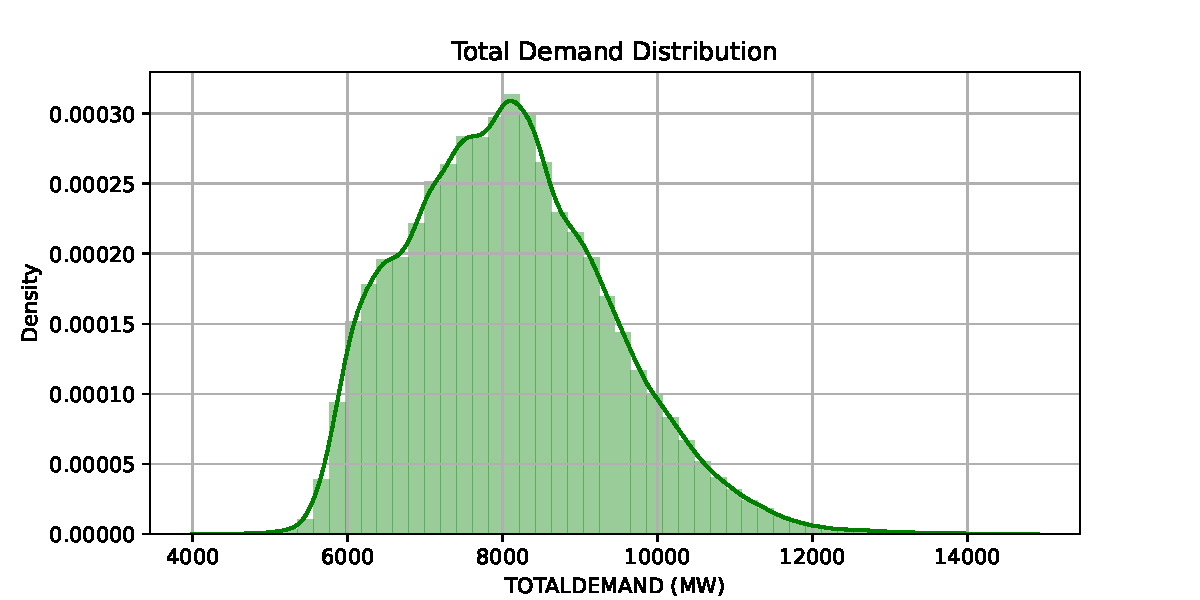
\includegraphics[width=1\linewidth,]{ZZSC9020_Group_Report_files/figure-latex/plot-density-curve-energy-demand-1} \caption{Total Demand Distribution}\label{fig:plot-density-curve-energy-demand}
\end{figure}

The distribution of energy demand is not symmetric, since an extended
right tail is plotted, which exceeds 14500 MW of demand. This indicates
there are occasional or a rare event when demand is significantly higher
than the average demand. This density curve implies the energy provider
and grid operators would need to be prepared for such rare high demand
periods. To maintain a stable supply of energy the energy providers may
need to have additional capacity in place.

\hypertarget{temperature-distribution}{%
\section{Temperature Distribution}\label{temperature-distribution}}

Figure \ref{fig:plot-temp-distribution} shows the density curve for the
distribution of NSW Temperature.

\begin{figure}[H]
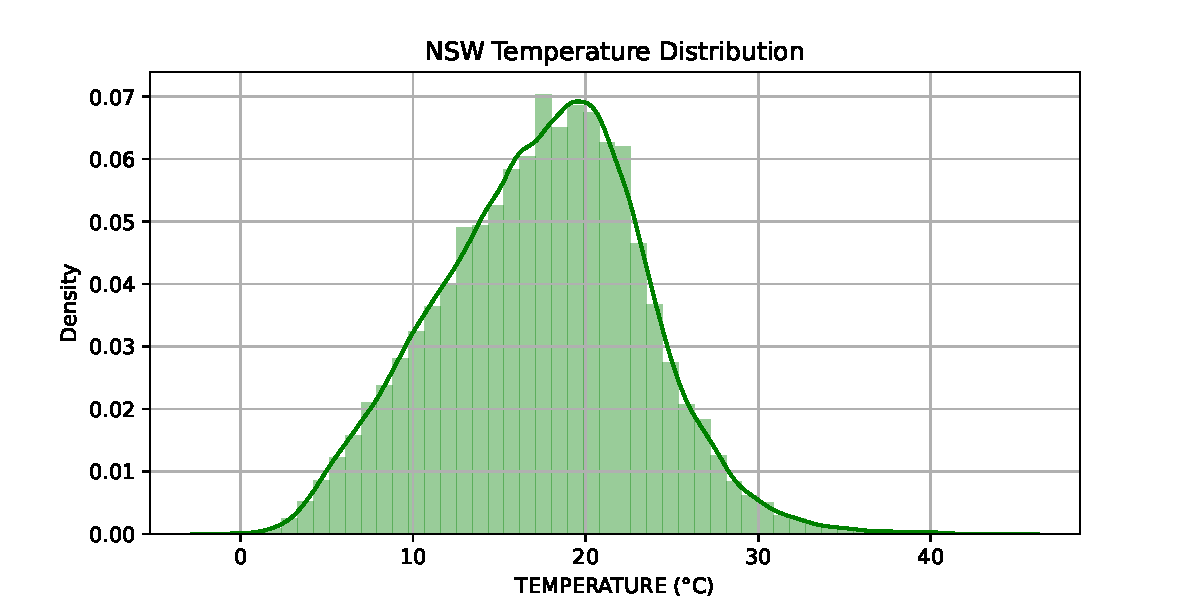
\includegraphics[width=1\linewidth,]{ZZSC9020_Group_Report_files/figure-latex/plot-temp-distribution-3} \caption{Temperature Distribution}\label{fig:plot-temp-distribution}
\end{figure}

The distribution of temperature is not symmetric, and it is right
skewed. The long tail to the right suggests majority of the data points
(lower temperatures) are less than the mean temperature of 17.40°C,
i.e.~concentrated to the left and few number of data points (higher
temperatures) are extending out to the right.

\hypertarget{relationship-between-energy-demand-and-temperature}{%
\section{Relationship Between Energy Demand and
Temperature}\label{relationship-between-energy-demand-and-temperature}}

The variables which relate to weather, i.e.~temperature, rainfall, solar
exposure, wind speed and humidity may have a significant impact on
energy demand. The inter-dependency between weather variables are
complex, but temperature is the key influential climatic variable
because it controls the atmospheric conditions. Therefore temperature
has the most important impact on energy demand (Vu et al. (2014)).

Graphs of observed energy demand and temperature are plotted and also a
Pearson correlation coefficient is measured to see if there is any
linear relationship between temperature and energy demand.

\begin{verbatim}
## array([<Axes: xlabel='DATETIME'>, <Axes: xlabel='DATETIME'>], dtype=object)
\end{verbatim}

\begin{figure}[H]
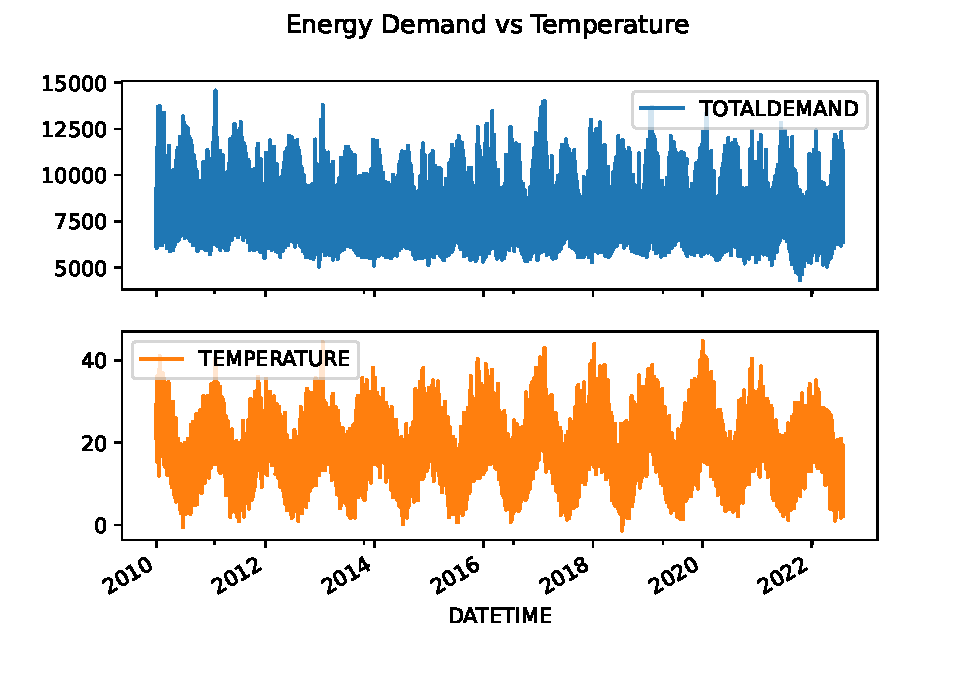
\includegraphics[width=1\linewidth,]{ZZSC9020_Group_Report_files/figure-latex/plot-energy-demand-temperature-by-year-5} \caption{Energy Demand vs Temperature}\label{fig:plot-energy-demand-temperature-by-year}
\end{figure}

\begin{verbatim}
## Correlation coefficient:
##               TEMPERATURE  TOTALDEMAND
## TEMPERATURE     1.000000     0.114347
## TOTALDEMAND     0.114347     1.000000
\end{verbatim}

Comparing the energy demand and temperature in Figure
\ref{fig:plot-energy-demand-temperature-by-year}, it is observed that as
temperature increases or decreases, the demand in energy consumption is
increasing. The correlation coefficient between them is 0.114 which
suggests a very weak linear relationship. But it is evident that
temperature greatly affects demand, but the relationship is non-linear.
A scatter plot confirms the non-linear relationship.

\begin{figure}[H]
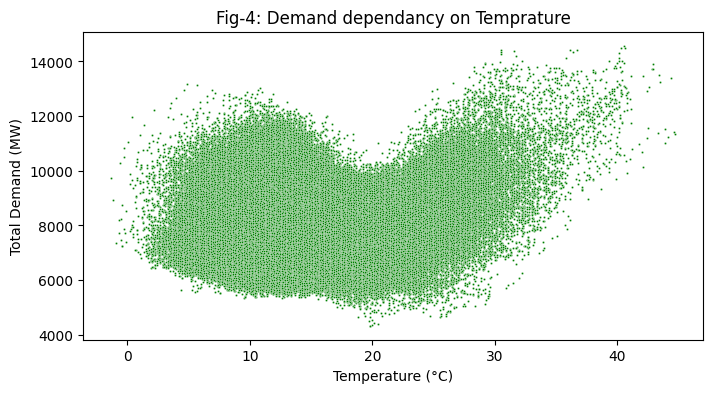
\includegraphics[width=1\linewidth,]{images/demand_dependency_on_temp} \caption{Energy Demand and Temperature Scatter Plot}\label{fig:plot-energy-demand-temperature-by-years}
\end{figure}

The demand dependency on temperature in Figure
\ref{fig:plot-energy-demand-temperature-by-years} clearly exhibits a
curve which indicates a non-linear relationship between demand and
temperature.

\hypertarget{components-of-time-series-seasonality-and-trend}{%
\section{Components of time series: Seasonality and
Trend}\label{components-of-time-series-seasonality-and-trend}}

Seasonality is a variation that occurs at specific regular intervals of
less than a year (e.g.~daily, weekly, monthly, or annually) and trend is
the presence of a long term increase or decrease in the sequence of data
(Auffarth (2021), NSW State of Environment (2022a)). In this part of
analyis given the datetime we tried to identify if there is a presence
of seasonality, treand and stationarity in the NSW historical energy
demand and temperature data.

Figure \ref{fig:plot-energy-demand-yearly-trend} shows the components of
time series.

\begin{figure}[H]
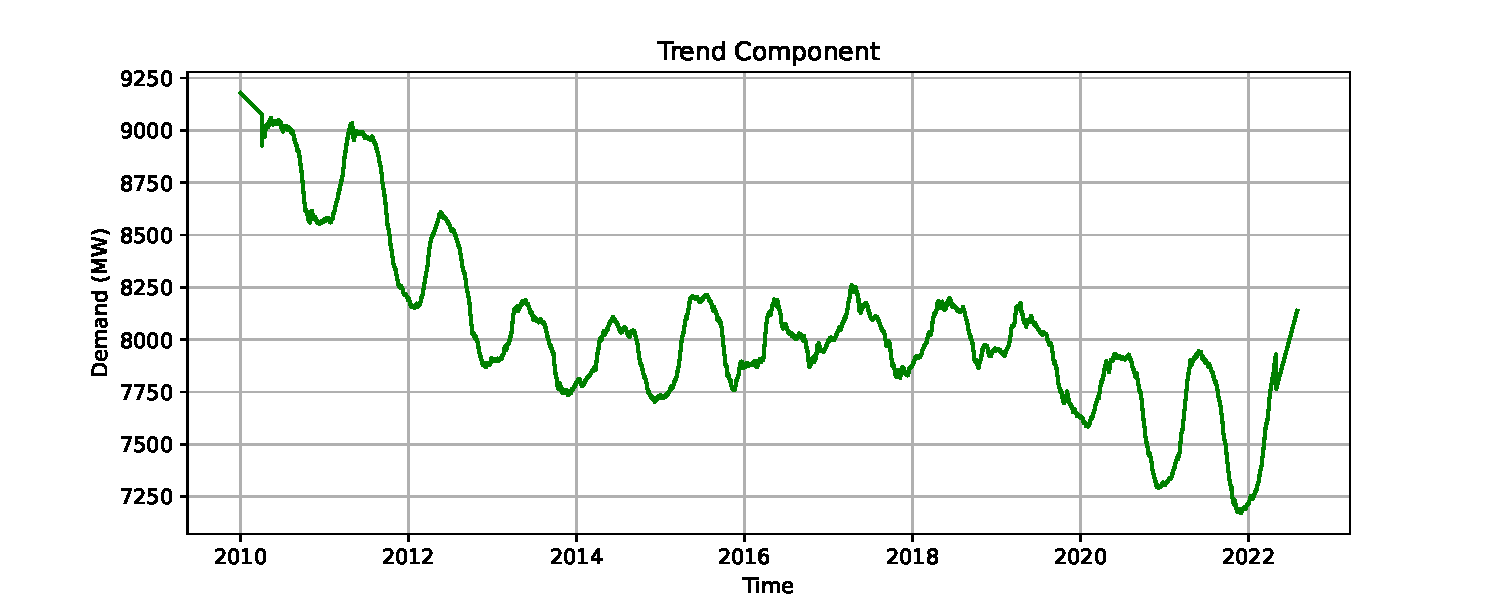
\includegraphics[width=1\linewidth,]{ZZSC9020_Group_Report_files/figure-latex/plot-energy-demand-yearly-trend-1} \caption{Energy Demand Yearly Trend}\label{fig:plot-energy-demand-yearly-trend}
\end{figure}

From the trend component in Figure
\ref{fig:plot-energy-demand-yearly-trend}, the demand for energy follows
a downward trend since year 2010 which supports the data, i.e.~the
energy consumption in NSW has decreased by 2\% over the past 10 years
(NSW State of Environment (2022b)). Each year, there are regular spikes
and dips in demand which indicate the presence of seasonality. For
further investigation, the data is split into monthly and daily demand
and can be represented in graphs.

\hypertarget{seasonality-by-month}{%
\subsection{Seasonality by month}\label{seasonality-by-month}}

\begin{figure}[H]
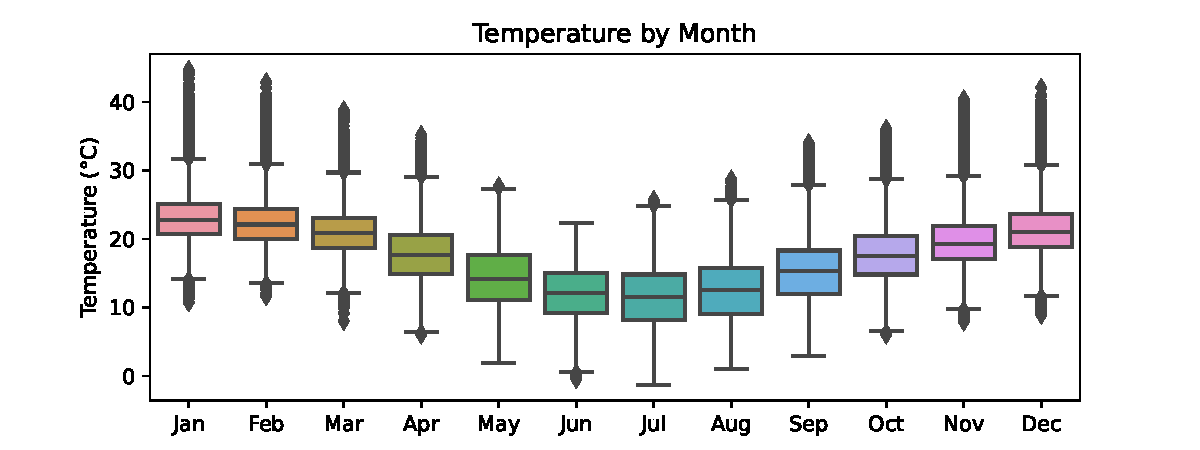
\includegraphics[width=1\linewidth,]{ZZSC9020_Group_Report_files/figure-latex/plot-energy-demand-temperature-monthly-3} \caption{Temperature And Energy Demand By Month}\label{fig:plot-energy-demand-temperature-monthly}
\end{figure}
\begin{figure}[H]
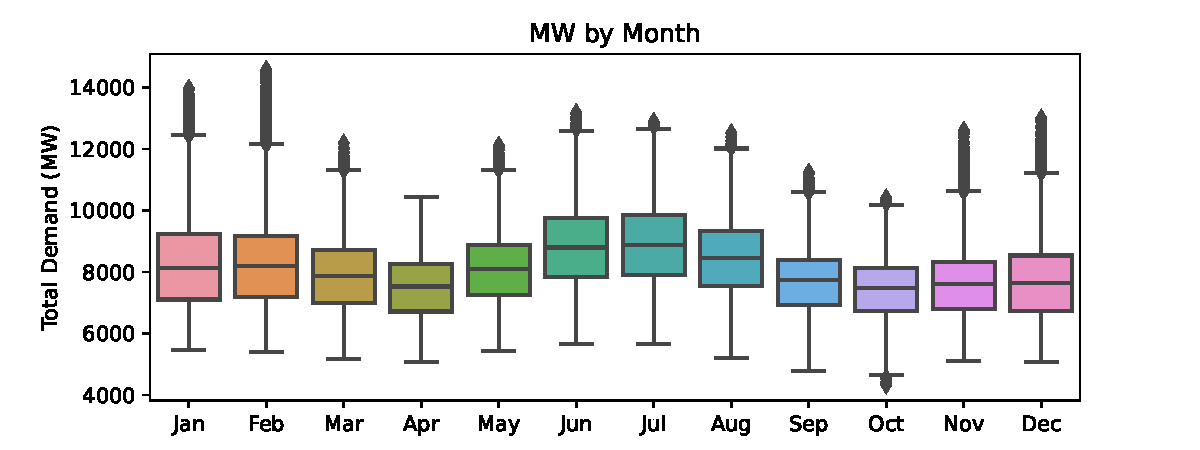
\includegraphics[width=1\linewidth,]{ZZSC9020_Group_Report_files/figure-latex/plot-energy-demand-temperature-monthly-4} \caption{Temperature And Energy Demand By Month}\label{fig:plot-energy-demand-temperature-monthly}
\end{figure}

In Australia, June, July and August are the coldest months during
winter. Summer has three hottest months, i.e.~December, January and
February. Spring has three transition months September, October and
November, and Autumn lasts for three months, i.e.~March, April and May.
The monthly energy demand in Figure
\ref{plot-energy-demand-temperature-monthly} shows that during Summer
and Winter the energy demand reaches its peak as people's usage of
air-conditioning in summer and heating system in winter increases. It
can be seen, during Spring and Autumn, the energy demand is lower, since
the temperature remains at an average temperature and the need for
heating or cooling homes decreases.

Year on year seasonal trend for the past twelve years from the year 2010
displays a repetitive seasonal trend in consumption of energy. This
implies a consistent and strong seasonal pattern in energy demand with
higher demand in winter and summer.

In Figure \ref{fig:year_to_year_seasonality_trend}, the seasonality
trend is depicted across successive years.

\begin{figure}[H]
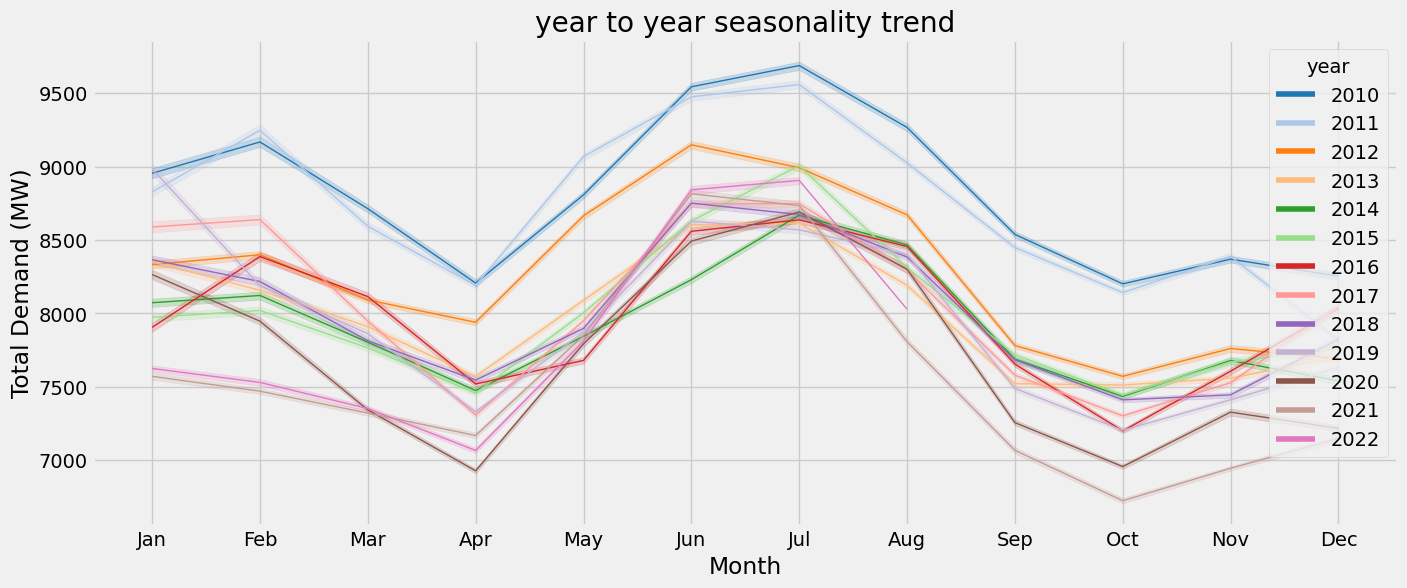
\includegraphics[width=1\linewidth,]{images/year_to_year_seasonality_trend} \caption{Year On Year Seasonality Trend}\label{fig:year_to_year_seasonality_trend}
\end{figure}

\hypertarget{average-monthly-demand}{%
\subsection{Average Monthly Demand}\label{average-monthly-demand}}

In Figure \ref{fig:year_to_year_seasonality_trend}, the distribution of
average monthly demand across the entire dataset is illustrated. The
figure reveals a distinct trend in monthly variations, providing
valuable insights into the cyclical nature of the demand.

\begin{figure}[H]
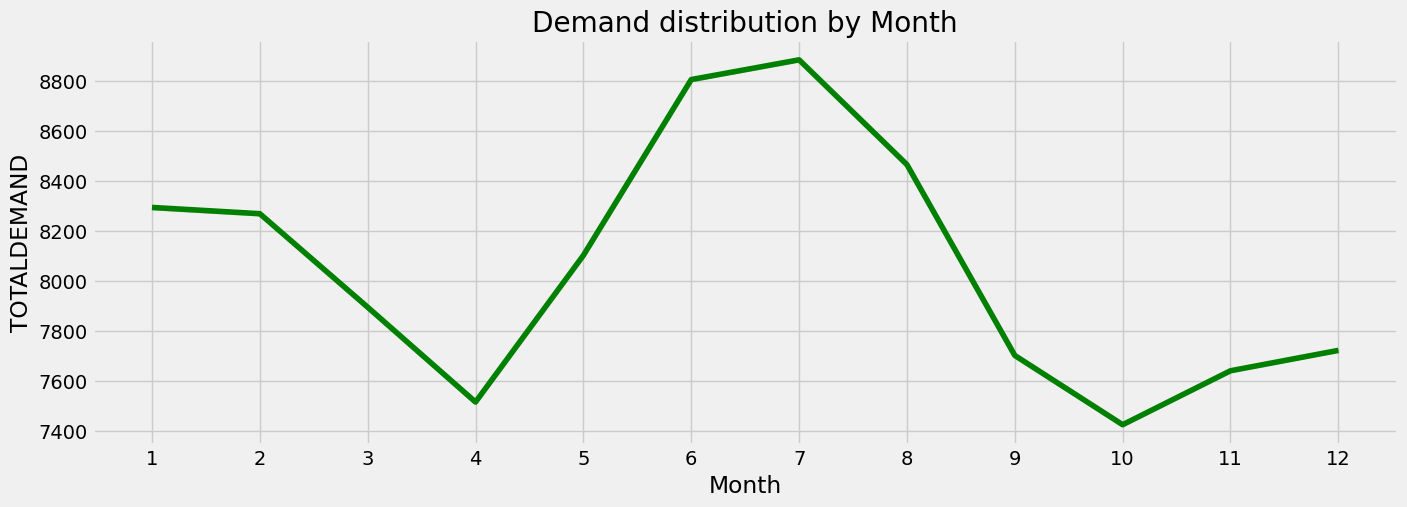
\includegraphics[width=1\linewidth,]{images/average_monthly_demand} \caption{Average Monthly Demand}\label{fig:average-monthly-demand}
\end{figure}

\hypertarget{seasonality-by-hour-of-the-day}{%
\subsection{Seasonality by hour of the
day}\label{seasonality-by-hour-of-the-day}}

The amount of energy being used is affected by many factors, but mostly
by temperature and time of the day.

\begin{figure}[H]
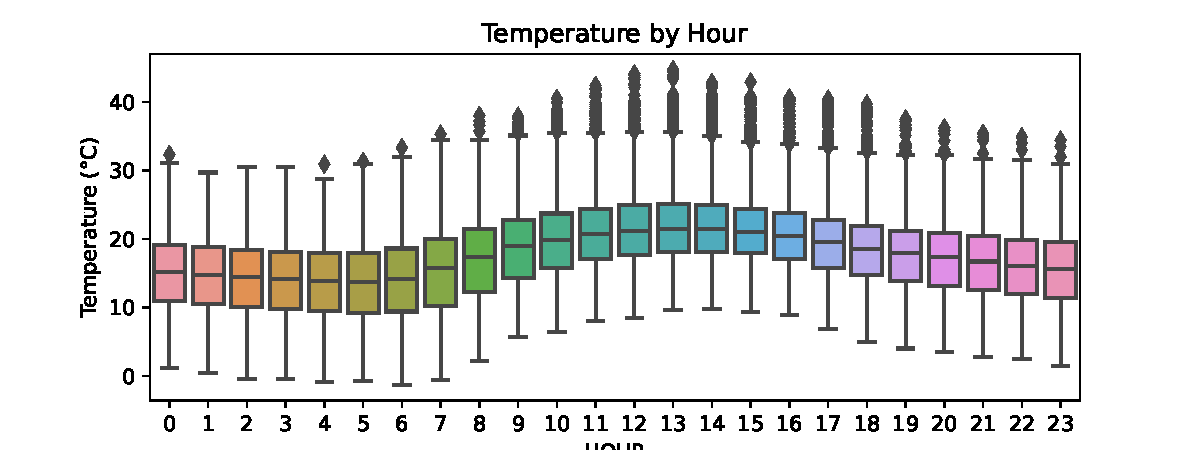
\includegraphics[width=1\linewidth,]{ZZSC9020_Group_Report_files/figure-latex/plot-demand-temperature-by-hour-1} \caption{Temperature and Energy Demand by Hour}\label{fig:plot-demand-temperature-by-hour}
\end{figure}
\begin{figure}[H]
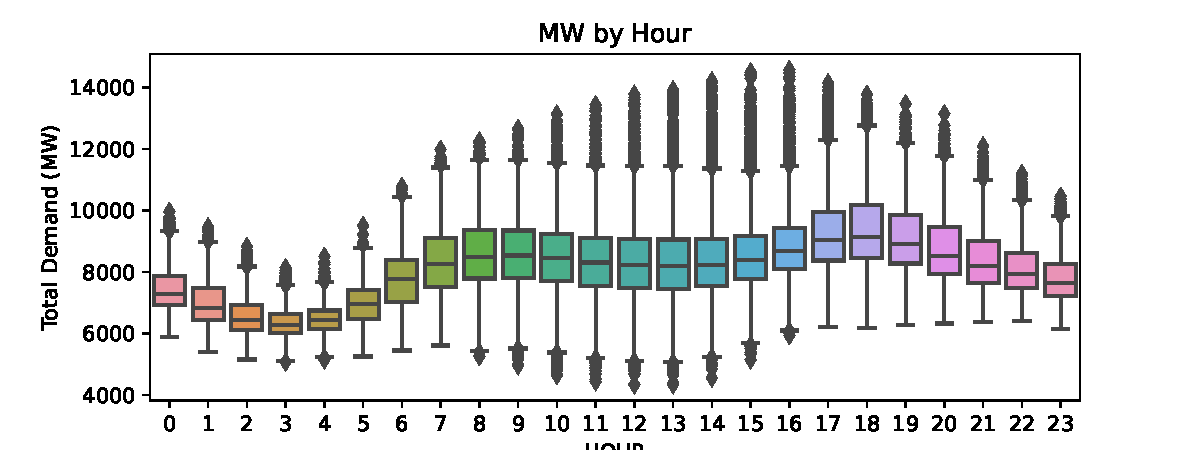
\includegraphics[width=1\linewidth,]{ZZSC9020_Group_Report_files/figure-latex/plot-demand-temperature-by-hour-2} \caption{Temperature and Energy Demand by Hour}\label{fig:plot-demand-temperature-by-hour}
\end{figure}

From Figure \ref{fig:plot-demand-temperature-by-hour}, on an average
day, it is observed the energy demand gradually increases through the
daytime as temperature outside increases. The demand picks at around 6pm
as people start getting home and use appliances when home. As the sun
and temperature decreases, demand starts dropping off and reaches to its
low between 2 and 3am in the morning because air-conditioning or heating
equipment are not being utilised.

\hypertarget{relationship-between-nsw-population-growth-and-energy-demand}{%
\section{Relationship Between NSW Population Growth and Energy
Demand}\label{relationship-between-nsw-population-growth-and-energy-demand}}

We assume that population has effect on energy demand, therefore, if
population increases, energy demand will increase too. To test this
assumption, we fit the regression line of energy demand against
estimated resident population.

\begin{figure}[H]
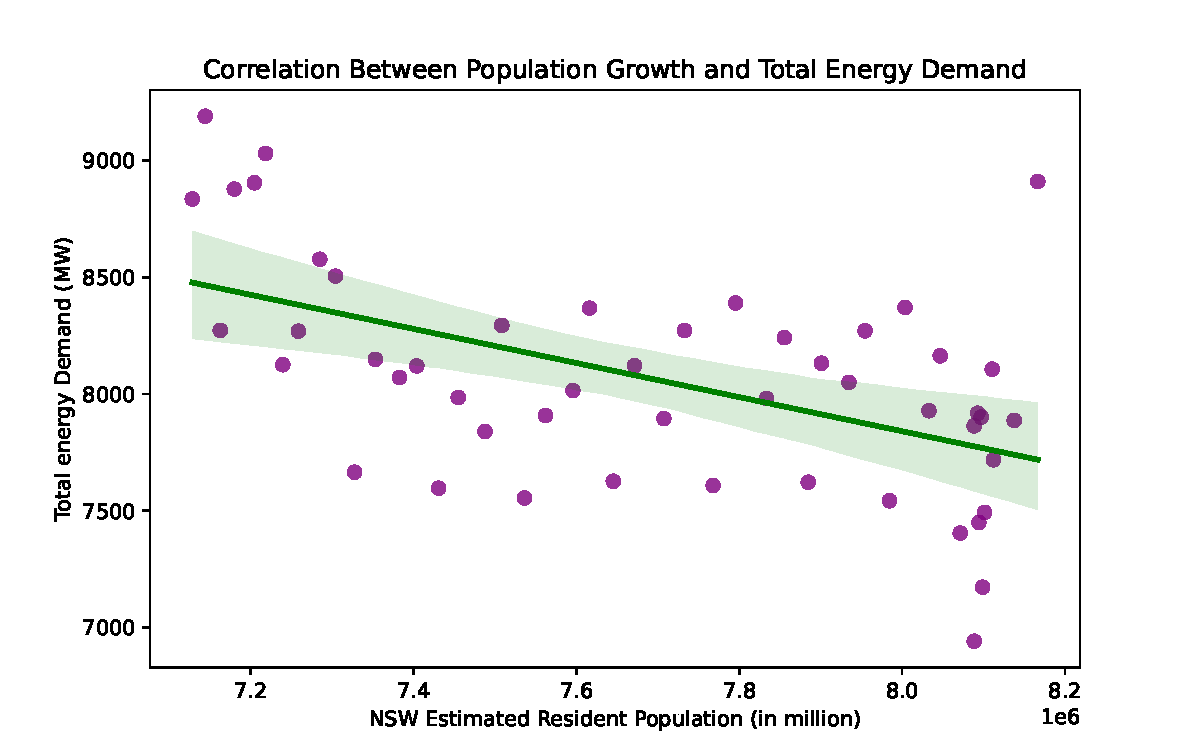
\includegraphics[width=1\linewidth,]{ZZSC9020_Group_Report_files/figure-latex/plot-demand-vs-population-5} \caption{Correlation Between Population Growth and Total Energy Demand}\label{fig:plot-demand-vs-population}
\end{figure}

As observed in Figure \ref{fig:plot-demand-vs-population}, the fitted
regression line of energy demand has a downward trend, demand decreases
as the population grows which also implies negative correlation. The
calculated correlation is -0.53. For several reasons energy demand and
population growth can exhibit negative correlation. Improved energy
efficient technology and infrastructure, advanced appliances and
industrial processes can significantly reduce the energy demand even if
the population grows. Shifts to new energy sources- shifts from fossil
fuel to more cleaner and efficient energy sources such as renewable
energy can significantly reduce the energy demand.

\hypertarget{relationship-between-energy-demand-and-energy-price}{%
\section{Relationship Between Energy Demand and Energy
Price}\label{relationship-between-energy-demand-and-energy-price}}

To investigate the relationship between energy demand and its price we
fit a regression line of energy demand against energy price.

\begin{figure}[H]
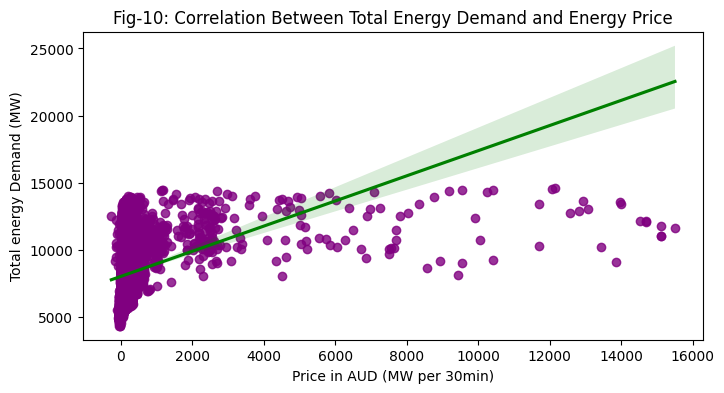
\includegraphics[width=1\linewidth,]{images/correlation_between_total_energy_demand_and_energy_price} \caption{Correlation Between Total Energy Demand and Energy Price}\label{fig:correlation-between-total-energy-demand-and-energy-price}
\end{figure}

The fitted regression line of energy demand in Figure
\ref{fig:correlation-between-total-energy-demand-and-energy-price}
follows an uptrend which also implies positive correlation between
energy demand and its price. The calculated correlation coefficient is
0.1345 implies a weak positive correlation. There are several reasons
for which energy demand could increase even though price increases. For
example, limited alternative to reduce the energy consumption in short
term period, Seasonal and Weather effect, regardless of the price people
are to consume more energy during winter and summer, income and economic
growth leads to higher consumption of energy even if the price
increases.

\hypertarget{relationship-between-energy-demand-and-holiday}{%
\section{Relationship Between Energy Demand and
Holiday}\label{relationship-between-energy-demand-and-holiday}}

Most often people are away from home while on holidays which results in
less consumption of energy. It is observed in Figure
\ref{fig:plot-energy-demand-holiday}, energy demand tends to go higher
when no holiday.

\begin{figure}[H]
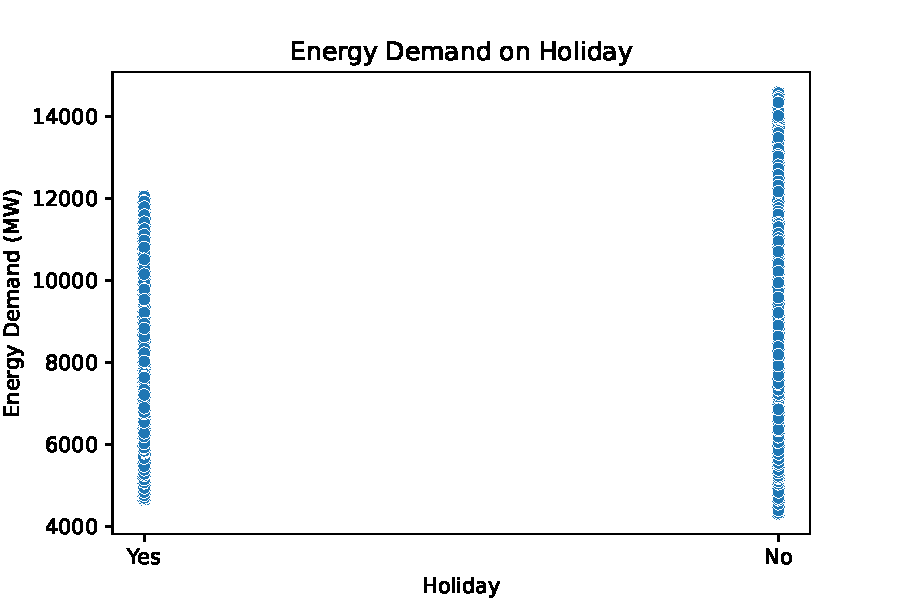
\includegraphics[width=1\linewidth,]{ZZSC9020_Group_Report_files/figure-latex/plot-energy-demand-holiday-1} \caption{Energy Demand on Holiday}\label{fig:plot-energy-demand-holiday}
\end{figure}

\hypertarget{s-analysis-results}{%
\chapter{Analysis and Results}\label{s-analysis-results}}

For the comparison of our model performance, we establish a benchmark
using the given demand forecast data and actual demand data. We consider
30 minutes frequency over the periods of 48 that gives a 24-hour
forecasting. The demand forecasting found to be highly accurate. Here
below the MAPE, MAE and RMSE scores are given.

\begin{longtable}[]{@{}rrr@{}}
\caption{Benchmark Evaluation Matrices}\tabularnewline
\toprule\noalign{}
MAPE & MAE & RMSE \\
\midrule\noalign{}
\endfirsthead
\toprule\noalign{}
MAPE & MAE & RMSE \\
\midrule\noalign{}
\endhead
\bottomrule\noalign{}
\endlastfoot
2.469\% & 204.027 & 280.450 \\
\end{longtable}

\hypertarget{results-from-initial-models}{%
\section{Results from Initial
Models}\label{results-from-initial-models}}

To forecast the energy demand, we initially consider three models:
Linear Regression, Multi-layer Perceptron and Random Forest.

In the first experiment, target variable is energy demand and inputs are
the temperature and time series features. The performances of different
models are shown below:

\begin{longtable}[]{@{}llrrr@{}}
\caption{\label{tab:eval-matrix-temp-time} Evaluation Matrices - with
Temperature and Time Series as Inputs}\tabularnewline
\toprule\noalign{}
Model & Data & MAPE & MAE & RMSE \\
\midrule\noalign{}
\endfirsthead
\toprule\noalign{}
Model & Data & MAPE & MAE & RMSE \\
\midrule\noalign{}
\endhead
\bottomrule\noalign{}
\endlastfoot
Linear Regression & train & 10.606\% & 855.533 & 1080.704 \\
& test & 11.422\% & 883.416 & 1146.064 \\
--------------------- & ----- & -------- & -------- & -------- \\
MLP & train & 10.899\% & 887.541 & 1117.268 \\
& test & 13.721\% & 1007.229 & 1222.413 \\
--------------------- & ----- & -------- & -------- & -------- \\
Random Forest & train & 6.987\% & 573.809 & 763.936 \\
& test & 11.321\% & 833.064 & 1083.929 \\
\end{longtable}

From Table \ref{tab:eval-matrix-temp-time}, it is seen that Linear
Regression model, with an MAPE error rate of 11.42\% and RMSE of 1146.06
on test data performs better than Multi-Layer Perceptron. But Random
Forest model outperforms both with an MAPE and RMSE score of 11.32\% and
1083.93, respectively.

With Linear regression there is an assumption a linear relationship
exists between the features and target variables. When plotting the
Energy Demand against Temperature, it was found there was a non-linear
relationship. Monthly, daily, weekly seasonality also exhibits
non-linear relationship with energy demand. Since the relationship is
non-linear, the linear model does not perform well with the complexity
of the data.

Here Random Forest performed better than Linear Regression because:

\begin{itemize}
\tightlist
\item
  data are not normally distributed
\item
  too many outliers in the data
\item
  Target-Features relationship are non-linear
\item
  Linear Regression struggle with complex feature interactions
\end{itemize}

Here Random Forest (RF) performs better than Multi-Layer Perceptron
because:

\begin{itemize}
\tightlist
\item
  RF deals with outliers very well in the data
\item
  less tuning for random forest
\item
  MLP struggle with complex feature interactions
\item
  Data are in a tabular format.
\end{itemize}

From the figure below, Figure
\ref{fig:actual-demand-vs-random-forest-prediction}, we can see that the
performance of Random Forest prediction is average. It mostly fails to
predict the demand when the demand is high or low, therefore,
seasonality was not captured.

\begin{figure}[H]
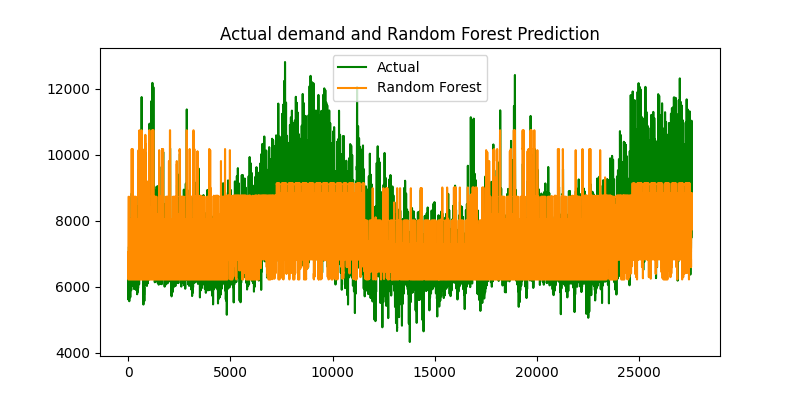
\includegraphics[width=1\linewidth,]{images/Actual_Demand_vs_Random_Forest_Prediction} \caption{Actual Demand vs Random Forest Prediction}\label{fig:actual-demand-vs-random-forest-prediction}
\end{figure}

\hypertarget{facebook-prophet-1}{%
\section{Facebook Prophet}\label{facebook-prophet-1}}

As a comparison, Facebook Prophet is also considered. In the first
model, to forecast energy demand, temperature, energy price, holiday and
time series features are used as regressors. This model produces a Mean
Absolute Percentage Error (MAPE) of 16.53. Again, a simple second model
is built without any regressor. It is found out that the second model
with a forecasting error rate of 9.79 (MAPE) outperforms the first
model.

\begin{longtable}[]{@{}lrrr@{}}
\caption{Forecasting error on test data set}\tabularnewline
\toprule\noalign{}
Facebook Prophet & MAPE & MAE & RMSE \\
\midrule\noalign{}
\endfirsthead
\toprule\noalign{}
Facebook Prophet & MAPE & MAE & RMSE \\
\midrule\noalign{}
\endhead
\bottomrule\noalign{}
\endlastfoot
Model-1 & 16.527 & 1233.650 & 1520.480 \\
Model-2 & 9.790 & 740.502 & 919.021 \\
\end{longtable}

\begin{figure}[H]
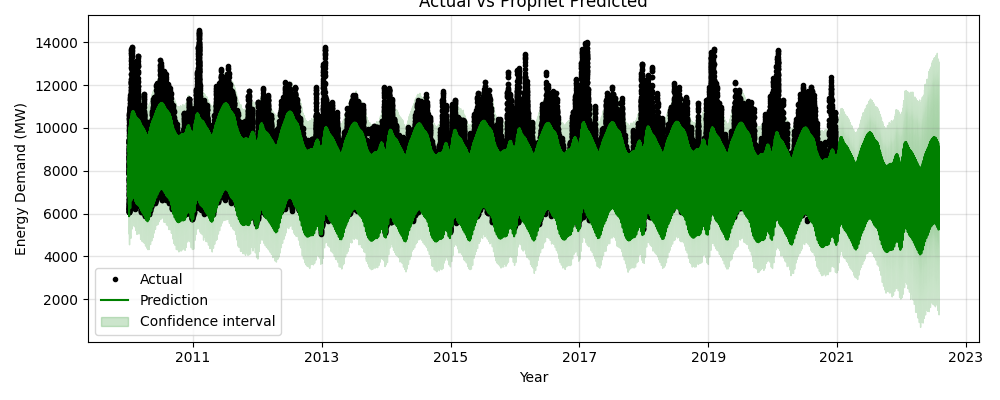
\includegraphics[width=1\linewidth,]{images/Actual_Demand_vs_Prophet_Prediction} \caption{Actual Demand vs Prophet Prediction}\label{fig:actual-demand-vs-prophet-prediction}
\end{figure}

\hypertarget{xgboost}{%
\section{XGBoost}\label{xgboost}}

In this final experiment, to forecast the energy demand by using
XGBoost, we include three more factors, price of energy, holiday and one
year lag as input. The reason for inclusions of one year of lag is that
we are also doing a one-year demand forecasting for the period of Aug
2022 to July 2023.

In our project, we adopt a 5-fold Time Series Split for
cross-validation. TimeSeriesSplit is particularly suited for time series
data, as it maintains the temporal order of observations. Unlike
standard k-fold cross-validation, Time Series Split ensures that each
training set is a superset of the one that precedes it. This aligns well
with our dataset, where autocorrelation is a key characteristic.

Fold 0: The first fold shows the smallest training set, in alignment
with TimeSeriesSplit's approach of adding surplus data to the initial
training partition.

Fold 1 to 4: Each subsequent fold illustrates that the training set
incorporates data from the preceding training sets and adds new data to
it, while the test set moves forward in time.

By visualizing these 5 folds, we can observe how each fold trains on an
increasingly larger set of past data to predict a future test set. This
enables a more realistic evaluation of our model's performance on
future, unseen data.

\begin{figure}[H]
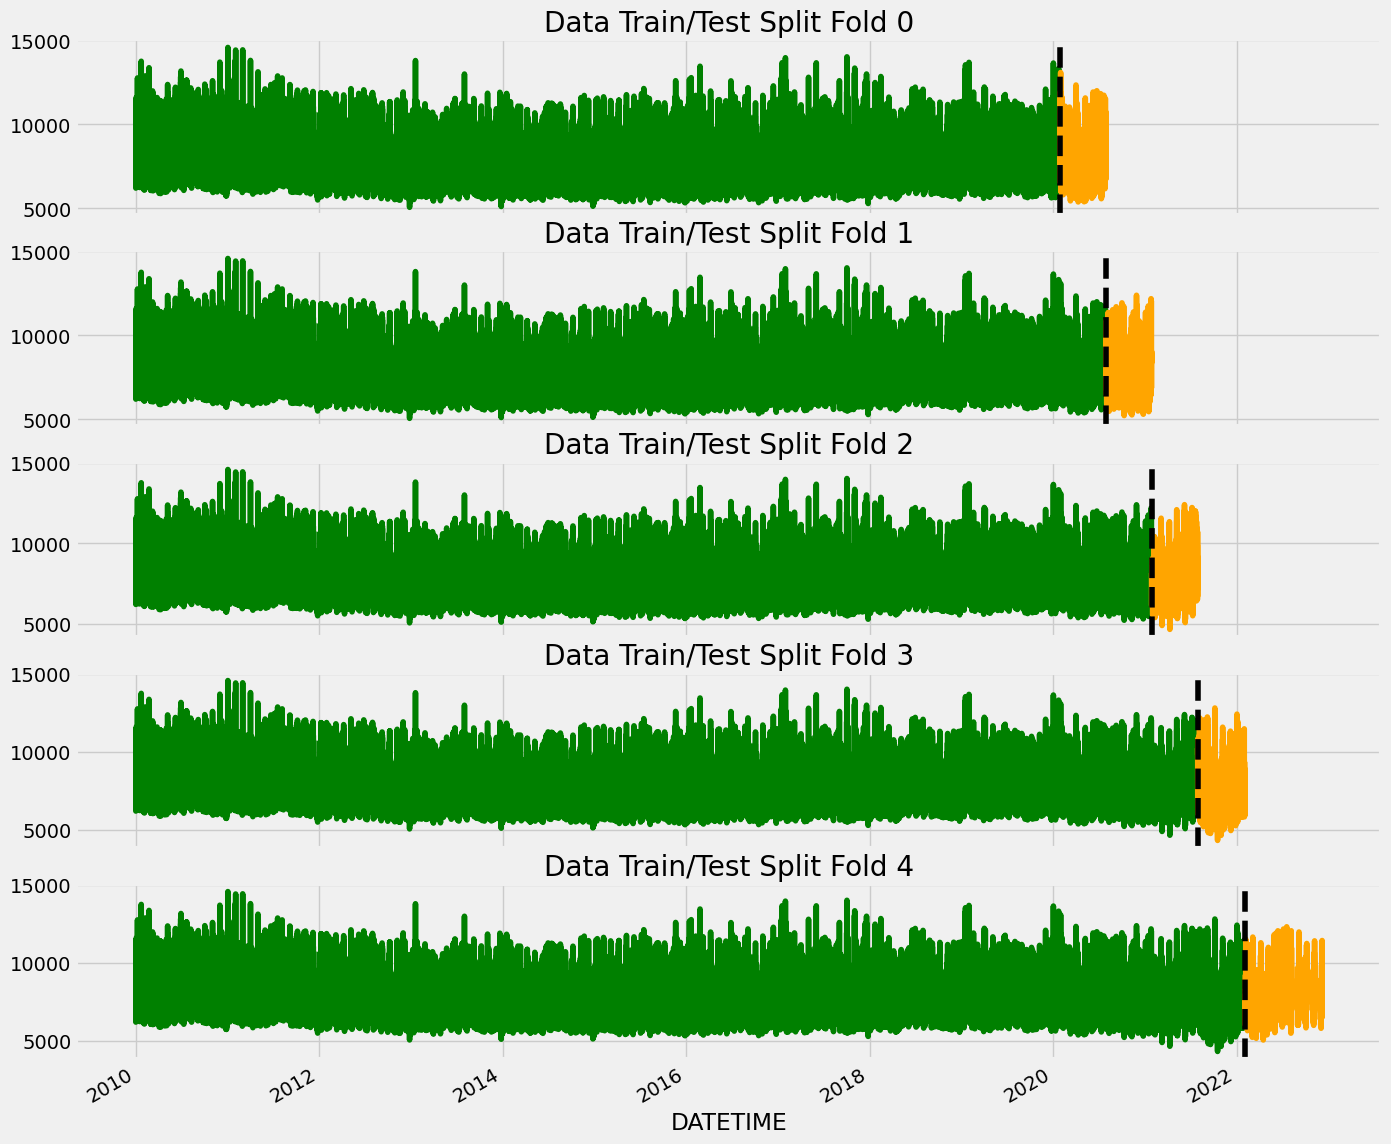
\includegraphics[width=1\linewidth,]{images/5folds TimeSeriesSplit} \caption{Five Folds Time Series Split}\label{fig:five-fold-img}
\end{figure}

By taking the lag we are using historical demand data from one year ago
and this would help us to capture the trend and pattern from the demand
data which may persist into the future. The performances matrices are
given below:

\begin{longtable}[]{@{}llrrr@{}}
\caption{Evaluation matrices- temperature, price, holiday and timeseries
features are factors}\tabularnewline
\toprule\noalign{}
Model & Data & MAPE & MAE & RMSE \\
\midrule\noalign{}
\endfirsthead
\toprule\noalign{}
Model & Data & MAPE & MAE & RMSE \\
\midrule\noalign{}
\endhead
\bottomrule\noalign{}
\endlastfoot
XGBoost & train & 5.87\% & 482.473 & 646.421 \\
& test & 7.03\% & 542.745 & 714.744 \\
\end{longtable}

As compared to our initial models in the first experiment, XGBoost
performed a lot better. It achieved a MAPE value of 7\% and RMSE score
of 714 on test dataset where for Random Forest they were 11\% and 1083,
respectively. The performance scores between training and test datasets
are not significantly different which indicates that this model has
overcome the overfitting issue. XGBoost forecasting will be more
reliable.

From the Figure: Actual demand and XGBoost Prediction, we see that it
failed to predict some of the extreme demand such as demand which was
over 1100MW and below 6000MW. But overall, it captured the most
variation in the energy demand.

Figure: Actual\_Demand\_vs\_XGBoost\_Prediction

\hypertarget{future-forecast-for-one-year}{%
\subsection{Future Forecast for one
year}\label{future-forecast-for-one-year}}

For next one year forecast we consider the period from Aug 2022 to July
2023. As we did not have future data, we considered the model
performances on the training dataset. Our XGBoost model achieved an MAPE
value of 5.76\% and RMSE score of 629.

From the figure below, we can see that model was quite good, capturing
the seasonal trend.

\begin{figure}[H]
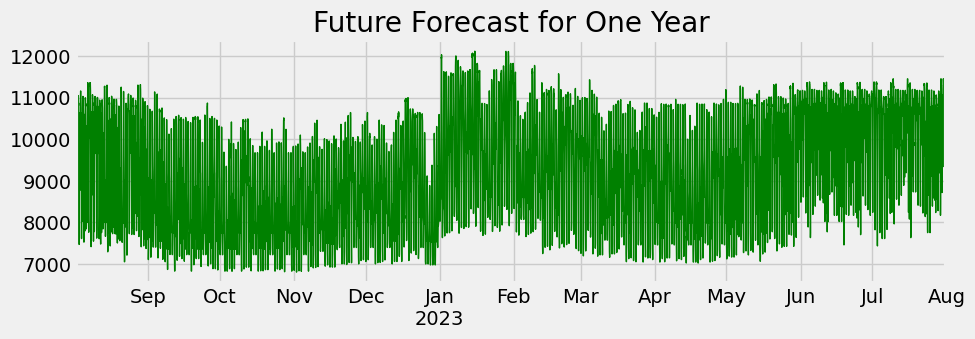
\includegraphics[width=1\linewidth,]{images/Future_Forecast_One_Year} \caption{Future Forecast For One Year}\label{fig:Future-Forecast-One-Year}
\end{figure}

\hypertarget{s-discussion}{%
\chapter{Discussion}\label{s-discussion}}

Although the Random Forest algorithm does significantly better than both
the Linear Regression and MLP models, it's worth noting that its
forecast error rate of 11.32\% still falls short when compared to the
benchmark error rate of 2.47\%. In a similar vein, Facebook Prophet
performs notably better than Random Forest, achieving a MAPE (Mean
Absolute Percentage Error) value of 9.8\% and an RMSE (Root Mean Square
Error) score of 740. However, even this model's error rate isn't as good
as the benchmark rate of 2.47\%.

As we looked for ways to improve upon these results, we considered
trying out another popular ensemble method known as XGBoost. Much like
Random Forest, XGBoost is grounded in decision tree algorithms and is
particularly good at capturing complex relationships and nuanced
patterns within the dataset. After undergoing several rounds of
hyperparameter tuning, after some trial and error, our XGBoost model
impressively reached a MAPE value of just 7\% and an RMSE score of 715.
These metrics were the best we could get among all the models we had
considered, leading us to adopt this XGBoost model as our final choice
for forecasting energy demand over the next year.

\begin{figure}[H]
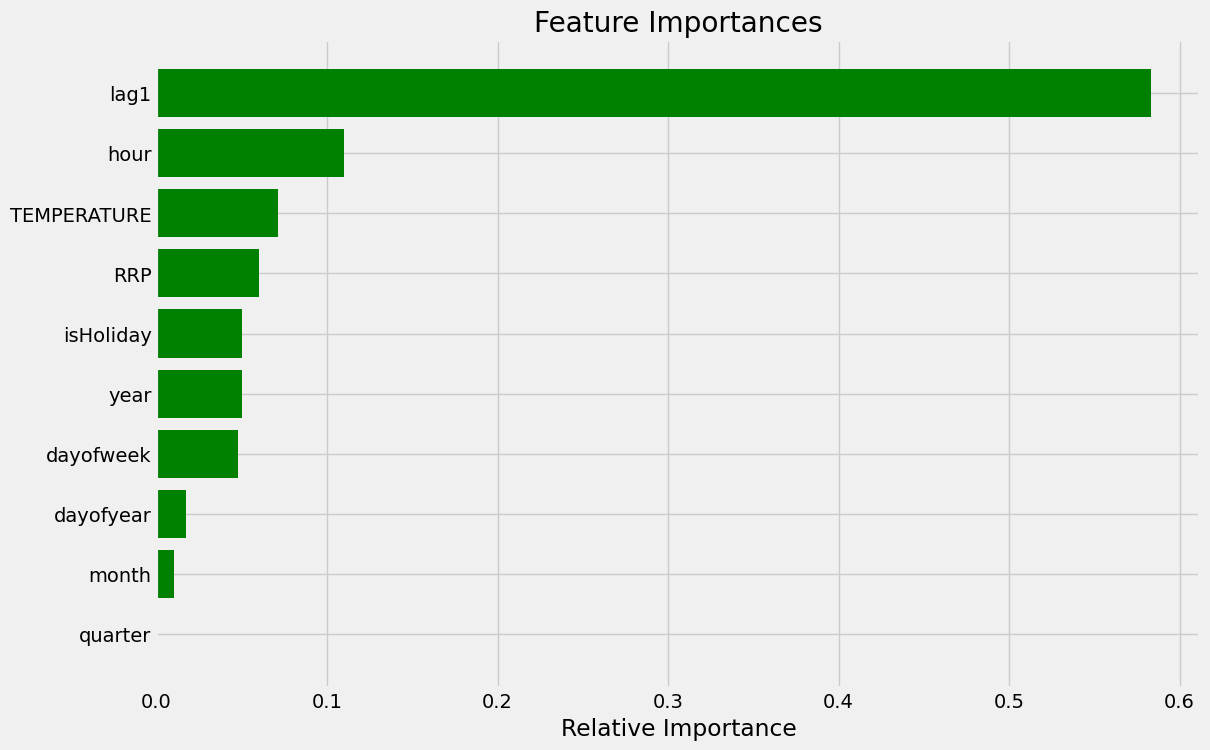
\includegraphics[width=1\linewidth,]{images/Feature_Importance} \caption{Feature Importance}\label{fig:Feature-Importance}
\end{figure}

In terms of feature importance, Figure \ref{fig:Feature-Importance} in
our report illustrates the most impactful variables according to our
final XGBoost model. Interestingly, the one-year lag and hourly lag
variables emerged as the two most influential factors. They were closely
followed by temperature, the price of energy, and the occurrence of
public holidays. These results serve to confirm one of the key
hypotheses of our project: namely, that variables such as temperature,
energy pricing, and public holidays have a meaningful impact on energy
demand. Therefore, these variables are worth considering in any future
energy demand forecasting efforts.

\hypertarget{s-conclusion}{%
\chapter{Conclusion and Further Issues}\label{s-conclusion}}

This paper has shown the impact of population, air temperature, seasons,
price of energy, holidays and several time series factors which impact
the energy demand. Population has a negative correlation with the energy
demand, whilst the other features have a positive impact on the energy
demand. Focusing on the top three features of highest importance,
i.e.~lag1, hour of the day, and temperature in the XGSBoost model, means
the previous years data, the hour of day and temperature had the most
importance when predicting energy demand for the next year.

Recognizing the inverse relationship between population growth and
energy demand observed in this study provides a valuable insight. The
government of New South Wales should focus on sustainable practices and
energy-efficient technologies to further reduce the environmental impact
associated with the increasing population densities, as highlighted
``Population density in NSW has also risen. In June 2020, there were an
average of 10.2 people per square kilometre -- a 7.4\% rise since 2015.
Across Greater Sydney, the average density reached almost 480 people per
square kilometre -- 41 more than in 2015.'' (NSW State of the
Environment (2023)).

There are initiatives which have been implemented by the NSW government
which

It is important to note, its crucial to emphasize the need for future
policies and strategies with the fact NSW government will need to manage
the expectation of the energy suppliers, i.e.~to keep the suppliers
contributing to the energy grid with a promise of continued business
prospects. The NSW government can take in consideration the effects of
global warming, ``Climate change is projected to increase temperatures
in Sydney with maximum temperatures projected to increase by 0.7°C by
2030'' (NSW environment and Heritage (2016)) and with these increases in
air temperature this would increase the energy demand.

Focusing on the time of day feature the peak energy demand happens
around 6pm, which is approximately when the sun sets, therefore solar
energy use can not be utilised to its maximum during peak demand
periods. The NSW Government can direct funding to Solar battery
providers and home owners to encourage the installation and use of
batteries for those high peak demand times. It has been found ``By
storing surplus energy during the day for use at night, batteries can
help you avoid using energy from the grid at peak times. With a battery
you can coast through the expensive times using battery-stored solar
energy that you harvested during the day.'' (The Institute of Community
Directors Australia (ICDA) (2023)). With this shift of power generation
and use, the current business for those energy suppliers could move into
the supply of batteries, and other alternate initiatives of energy to
the market and to keep businesses in the market and profitable.

When focusing on the model, and improving the forecast model, more
historical data would be beneficial to improve the forecast model. Other
suggestions would be to include other features into the model which
would contribute to the decrease of energy, and factors leading to the
decrease in demand and ensure the NSW Government has a sustainable
energy supply and demand for the population of NSW.

\hypertarget{references}{%
\chapter*{References}\label{references}}
\addcontentsline{toc}{chapter}{References}

\hypertarget{refs}{}
\begin{CSLReferences}{0}{0}
\leavevmode\vadjust pre{\hypertarget{ref-identify-trend-and-seasonality}{}}%
Auffarth, B. (2021) {`Machine learning for time-series with python'}.
Packt. Available at:
\url{https://subscription.packtpub.com/book/data/9781801819626/2/ch02lvl1sec11/identifying-trend-and-seasonality}.

\leavevmode\vadjust pre{\hypertarget{ref-abs-population}{}}%
Australian Bureau of Statistics ({[}no date{]}) {`National, state and
territory population'}. Available at:
\url{https://www.abs.gov.au/statistics/people/population/national-state-and-territory-population/latest-release}.

\leavevmode\vadjust pre{\hypertarget{ref-aemo-aggregated-price-demand}{}}%
Australian Energy Market Operator ({[}no date{]}) {`Aggregated price and
demand data'}. Available at:
\url{https://aemo.com.au/en/energy-systems/electricity/national-electricity-market-nem/data-nem/aggregated-data}.

\leavevmode\vadjust pre{\hypertarget{ref-elsayed-2021}{}}%
Elsayed, S, Thyssens, D, Rashed, A, Jomaa, HS \& Schmidt-Thieme, L
(2021) {`{Do We Really Need Deep Learning Models for Time Series
Forecasting?}'} Available at: \url{https://arxiv.org/abs/2101.02118}.

\leavevmode\vadjust pre{\hypertarget{ref-Javanmard-et-al-2023-energy-demand-forecast}{}}%
Emami Javanmard, M. and Ghaderi, S.F. (2023) {`Energy demand forecasting
in seven sectors by an optimization model based on machine learning
algorithms'}. \emph{Sustainable Cities and Society} 95, p. 104623.
Available at:
\url{https://www.sciencedirect.com/science/article/pii/S2210670723002342}.

\leavevmode\vadjust pre{\hypertarget{ref-github-facebook}{}}%
GitHub, Facebook Open Source (2021) {`{Forecasting at scale}'}.
Available at: \url{https://facebook.github.io/prophet/}.

\leavevmode\vadjust pre{\hypertarget{ref-zabel-G-2009}{}}%
Graham Zabel (2009) {`{Peak People: The Interrelationship between
Population Growth and Energy Resources}'}. Available at:
\url{https://www.resilience.org/stories/2009-04-20/peak-people-interrelationship-between-population-growth-and-energy-resources/}.

\leavevmode\vadjust pre{\hypertarget{ref-iea-world-energy-outlook-2016}{}}%
IEA (2016) {`World energy outlook 2016'}. Available at:
\url{https://www.iea.org/reports/world-energy-outlook-2016}.

\leavevmode\vadjust pre{\hypertarget{ref-emami-2023}{}}%
Majid Emami Javanmard, S.F. Ghaderi (2023) {`{Energy demand forecasting
in seven sectors by an optimization model based on machine learning
algorithms}'}. Available at:
\url{https://www.sciencedirect.com/science/article/pii/S2210670723002342}.

\leavevmode\vadjust pre{\hypertarget{ref-environment-2023}{}}%
Minister for Planning and Public Spaces (2023) {`{Analysis and
Forecasting of Monthly Electricity Demand Time Series Using
Pattern-Based Statistical Methods}'}. Available at:
\url{https://www.nsw.gov.au/media-releases/sustainable-building-reforms\#:~:text=The\%20new\%20standard\%20cuts\%20thermal}.

\leavevmode\vadjust pre{\hypertarget{ref-nsw-climate-change-fact-sheet}{}}%
NSW environment and Heritage (2016) {`{Fact Sheet - Climate Change in
NSW}'}. Available at:
\url{https://www.environment.nsw.gov.au/-/media/OEH/Corporate-Site/Documents/Climate-change/climate-change-fact-sheet-160595.pdf}.

\leavevmode\vadjust pre{\hypertarget{ref-nsw-epa-status-trend}{}}%
NSW State of Environment (2022a) {`Energy consumption'}. Available at:
\url{https://www.soe.epa.nsw.gov.au/all-themes/human-settlement/energy-consumption\#final-energy-consumption-status-and-trends}.

\leavevmode\vadjust pre{\hypertarget{ref-nsw-of-environment-2022}{}}%
NSW State of Environment (2022b) {`{Energy Consumption}'}. Available at:
\url{https://www.soe.epa.nsw.gov.au/all-themes/human-settlement/energy-consumption\#final-energy-consumption-status-and-trends}.

\leavevmode\vadjust pre{\hypertarget{ref-nsw-population}{}}%
NSW State of the Environment (2023) {`{Population - Population growth is
a key driver of changes to the environment caused by humans}'}.
Available at:
\url{https://www.soe.epa.nsw.gov.au/all-themes/drivers/population}.

\leavevmode\vadjust pre{\hypertarget{ref-pelka-p-2023}{}}%
Pawel Pelka (2023) {`{Analysis and Forecasting of Monthly Electricity
Demand Time Series Using Pattern-Based Statistical Methods}'}. Available
at: \url{https://www.mdpi.com/1996-1073/16/2/827}.

\leavevmode\vadjust pre{\hypertarget{ref-perle-2023-predicting-power}{}}%
Perle (2023) {`Predicting power: How machine learning is enhancing
energy demand forecasting'}. Available at:
\url{https://www.perle.com/articles/predicting-power-how-machine-learning-is-enhancing-energy-demand-forecasting-40196905.shtml}.

\leavevmode\vadjust pre{\hypertarget{ref-battery-storage-systems}{}}%
The Institute of Community Directors Australia (ICDA) (2023) {`{Battery
Storage Systems}'}. Available at:
\url{https://communitydirectors.com.au/help-sheets/battery-storage-systems\#:~:text=By\%20storing\%20surplus\%20energy\%20during,you\%20harvested\%20during\%20the\%20day.}

\leavevmode\vadjust pre{\hypertarget{ref-eia-2020-global-electricity-consumption-population}{}}%
U.S Energy Information Administration (2020) {`Global electricity
consumption continues to rise faster than population'}. Available at:
\url{https://www.eia.gov/todayinenergy/detail.php?id=44095}.

\leavevmode\vadjust pre{\hypertarget{ref-vu-et-al-2014-climate-variables-energy-demand}{}}%
Vu, D.H., Muttaqi, K.M. and Agalgaonkar, A.P. (2014) {`Assessing the
influence of climatic variables on electricity demand'}. in \emph{2014
IEEE PES general meeting \textbar{} conference \& exposition}., pp.
1--5. Available at: \url{https://ieeexplore.ieee.org/document/6939377}.

\leavevmode\vadjust pre{\hypertarget{ref-wikipedia-mape}{}}%
Wikipedia, the free encyclopedia (2023a) {`{Mean absolute percentage
error}'}. Available at:
\url{https://en.wikipedia.org/wiki/Mean_absolute_percentage_error}.

\leavevmode\vadjust pre{\hypertarget{ref-wikipedia-rms}{}}%
Wikipedia, the free encyclopedia (2023b) {`{Root-mean-square
deviation}'}. Available at:
\url{https://en.wikipedia.org/wiki/Root-mean-square_deviation}.

\leavevmode\vadjust pre{\hypertarget{ref-Wolde-Rufael-2006-electricity-consumption-economic-growth}{}}%
Wolde-Rufael, Y. (2006) {`Electricity consumption and economic growth: A
time series experience for 17 african countries'}. \emph{Energy Policy}
34(10), pp. 1106--1114. Available at:
\url{https://www.sciencedirect.com/science/article/pii/S0301421504003155}.

\end{CSLReferences}

\bibliographystyle{elsarticle-harv}
\bibliography{references}

\hypertarget{appendix}{%
\chapter*{Appendix}\label{appendix}}
\addcontentsline{toc}{chapter}{Appendix}

\hypertarget{sourcing-public-holidays}{%
\section{Sourcing Public holidays}\label{sourcing-public-holidays}}

We did not take in consideration the local holidays since it changes
depending on the council, and the current demand and temp data sets do
not have local council data.

\hypertarget{source-of-data}{%
\subsection{Source of data}\label{source-of-data}}

\begin{itemize}
\tightlist
\item
  \href{https://date.nager.at/PublicHoliday/Australia/2011}{2011:
  Nager.Date - Public Holidays in Australia 2011}
\item
  \href{https://date.nager.at/PublicHoliday/Australia/2012}{2012:
  Nager.Date - Public Holidays in Australia 2012}
\item
  \href{https://www.industrialrelations.nsw.gov.au/public-holidays/public-holidays-in-nsw/nsw-public-holidays-2013-2015/}{2013-2015:
  NSW Public Holidays 2013-2015}
\item
  \href{https://www.industrialrelations.nsw.gov.au/public-holidays/public-holidays-in-nsw/nsw-public-holidays-2019-2020/}{2019-2020:
  NSW Public Holidays 2019-2020}
\item
  \href{https://data.gov.au/data/dataset/australian-holidays-machine-readable-dataset}{2014-2024:
  Australian Public Holidays Dates Machine Readable Dataset}
\end{itemize}

\hypertarget{git-repository}{%
\section{Git Repository}\label{git-repository}}

\begin{itemize}
\tightlist
\item
  \href{https://github.com/van-hai-ho/ZZSC9020_Project_Group_K/blob/main/src/README.md}{Scripts
  for merging data, exploratory, and models}
\item
  \href{https://github.com/van-hai-ho/ZZSC9020_Project_Group_K/tree/main/data}{All
  source data files, and merged data files}
\item
  \href{https://github.com/van-hai-ho/ZZSC9020_Project_Group_K/tree/main/report/Group_Report}{Report
  files}
\end{itemize}







\end{document}

